\documentclass{article}
\usepackage{authblk}
\usepackage[utf8]{inputenc}
\usepackage[T1]{fontenc}
\usepackage[pdftex]{graphicx}
\usepackage{amsmath,amssymb,color}
\usepackage{mathtools}
\usepackage{natbib}
\usepackage{palatino}
\usepackage{float}
\usepackage{placeins}
\usepackage{multirow}
\usepackage{booktabs}
\usepackage{subcaption}
\usepackage{nicefrac}
\usepackage{siunitx}
\usepackage{appendix}
\usepackage{xspace}
\usepackage[hidelinks]{hyperref}

\usepackage{todonotes}
% \usepackage[disable]{todonotes}
\definecolor{todoblue}{RGB}{30,90,220}
\definecolor{reviewred}{RGB}{200,30,30}
\newcommand{\TODOc}[1]{\todo[inline,color=todoblue!18,bordercolor=todoblue,linecolor=todoblue]{\textbf{\textcolor{todoblue}{TODO:}} #1}}
\newcommand{\REVIEWc}[1]{\todo[inline,color=reviewred!16,bordercolor=reviewred,linecolor=reviewred]{\textbf{\textcolor{reviewred}{REVIEW:}} #1}}

\clubpenalty=10000
\widowpenalty=10000
\displaywidowpenalty=3000
\predisplaypenalty=3000
\postdisplaypenalty=2000
\setlength{\emergencystretch}{3em}
\raggedbottom
\captionsetup{justification=raggedright,singlelinecheck=false}
\setlength{\textwidth}{6.5in}
\setlength{\oddsidemargin}{0.in}
\setlength{\topmargin}{-10pt}
\setlength{\headsep}{0in}
\setlength{\textheight}{8.95in}
\sisetup{detect-all,range-units = single,range-phrase = --}
\DeclareSIUnit\PSU{PSU}
\newcommand{\Linf}{L_\infty}
\newcommand{\Lone}{L_1}
\newcommand{\Ltwo}{L_2}
\newcommand{\interior}{\text{interior}}
\newcommand{\partialset}{\text{partial}}
\newcommand{\fracmpas}{\chi}
\newcommand{\hkm}{h}
\newcommand{\hR}{h_{\mathrm{ROMS}}}
\newcommand{\hM}{h_{\mathrm{MPAS}}}
\newcommand{\MPAS}{\textsc{MPAS}\xspace}
\newcommand{\ROMS}{\textsc{ROMS}\xspace}
\newcommand{\MOAB}{\textsc{MOAB}\xspace}
\newcommand{\zmpas}{z^{*}}
\newcommand{\hRatio}{\varrho}

%
\title{Enhanced Submesoscale Feature Resolution in Multiscale Ocean Simulations}
\author[1]{Authors**}
\affil[1]{Institutions}
\date{\today}
\begin{document}
\maketitle
\TODOc{Author metadata: Replace placeholder for authors and institution fields.}
%

%
\begin{abstract}
Global ocean models must limit horizontal resolution, even when using regional refinement, to make climate-length integrations computationally tractable. Regional downscaling addresses this constraint by representing selected processes, in a limited region, at finer resolution within a global modeling framework, but it requires the consistent transfer of three-dimensional state fields between global and regional model components. Differences in horizontal mesh topology and characteristic scales, together with differences in vertical coordinate systems, complicate the construction of a verifiably accurate coupler. We present a scalable global \MPAS$\rightarrow$\ROMS regional model tensor-product transfer for multiscale boundary conditions that applies a consistent, property-preserving horizontal map independently at each vertical level over the common mesh support, followed by a conservative vertical remap that preserves column integrals of salinity, temperature, and velocity fields. Tests using a smooth analytic field and daily-mean ocean states show decreasing error as the \ROMS mesh is refined, followed by error saturation when \MPAS to \ROMS characteristic lengths are about $0.2$. These convergence results identify regional grid resolutions that meet a prescribed accuracy target at lower computational cost. We assess the resulting regional fields in deep-ocean North Atlantic and Gulf Stream domains and in coastal and estuarine applications in the Bay of Bengal and Chesapeake Bay, where the downscaled fields represent variability at scales finer than those resolved by the global model, including submesoscale structure where supported by the regional mesh resolution and forcing. Together, these results demonstrate the feasibility of the proposed transfer method for multiscale ocean downscaling across open-ocean, coastal, and estuarine settings with possible extensions to both online one-way and two-way setups.
\end{abstract}
%
\vspace{0.5em}
\noindent\textbf{Keywords:} multiscale ocean coupling; volumetric remapping;
\MPAS{}-Ocean; \ROMS.

%
\listoftodos[\textbf{Outstanding TODO (blue) and REVIEW (red) notes}]
\clearpage

%

\FloatBarrier
\section{Introduction}
Global ocean models are integrated over decadal time scales, which constrains the horizontal and temporal resolution that can be used in global simulations. As a result, many dynamically important processes are only partly resolved or remain unresolved, including mesoscale eddies with scales of approximately 10--100 km, mixed-layer instabilities, and submesoscale fronts. These processes influence heat transport, circulation, restratification, and tracer exchange \citep{boccaletti2007mixed,foxkemper2008mle,thomas2008submesoscale,taylor2023submesoscale}. Their effects must therefore be represented through parameterizations whose behavior strongly depends on model resolutions \citep{hallberg2013using}, the consequences of which are particularly apparent near coastal fronts, river plumes, shelf breaks, and western boundary currents, where circulation and tracer pathways can remain sensitive to grid spacing \citep{chassignet2017impact}.

One-way global-to-regional coupling provides a means of increasing resolution over a selected regional domain without applying that restrictive resolution specification throughout the global ocean. Here, the ocean component of the Energy Exascale Earth System Model (E3SM)~\citep{golaz2019e3sm}, \MPAS ocean \citep{ringler2013multi,hoch2020MPAS}, supplies the evolving large-scale state, including the regional initial condition and lateral boundary fields. The Regional Ocean Modeling System (\ROMS)~\citep{shchepetkin2005regional} is then integrated on a finer regional grid, and coupled to the global ocean system to receive consistent conditions. The regional domain can include bathymetry and coastline geometry that are not fully resolved by the \MPAS mesh, thereby improving the representation of local circulation and nearshore structure. Grid refinement alone, however, does not add the information absent from the global solutions. For example, conservative downscaling alone cannot recover unresolved fronts, stratification, and boundary variability, and this is a result of the regional model evolution of state with the right forcing conditions.
%develops must be interpreted separately from the information that the  \MPAS actually supplied: refining the regional grid cannot reconstruct fronts, stratification, or boundary variability absent from the  \MPAS state.


Regional nesting and downscaling methods have been developed previously for coupled global model settings. \citet{penven2006embedding} described a one-way \ROMS embedding procedure in which initial and lateral boundary conditions were derived from a coarser parent solution, while \citet{mason2010nesting} extended offline nesting methods to regional grids. Later work considered online and two-way approaches, including feedback from the regional model to the parent domain \citep{debreu2008embedding,debreu2012nesting}. These methods established practical approaches for ocean nesting, but the present problem differs in several respects. \MPAS ocean model uses a variable-resolution unstructured horizontal mesh, whereas \ROMS uses a structured, curvilinear grid and terrain-following vertical coordinates. Coupling the models therefore requires transfers that are consistent not only in the horizontal plane, but also across the three-dimensional water-column geometries during the entire coupled transient simulation. \TODOc{Need to add more details on how this work differs from the previous ones}


%SCRIP introduced first- and second-order conservative remapping on spherical grids~\citep{jones1999scrip}, while the TempestRemap linear-map framework generalized consistency and conservation to arbitrary meshes and orders~\citep{ullrich2015arbitrary,ullrich2016tempestremap}. High-order regridding between generalized ocean vertical coordinates addressed the axial part of the problem~\citep{white2009highorder}; applying horizontal and vertical transfer together still requires a consistent representation of the two three-dimensional column geometries.

General coupling frameworks such as ESMF provide component interfaces, field definitions, grid descriptions, and regridding services for Earth-system applications \citep{hill2004esmf}. MCT provides parallel data structures and communication patterns for coupled models \citep{larson2005mct}, and its use in COAWST supports coupled regional ocean--atmosphere--wave--sediment simulations \citep{warner2010coawst}. We instead build on the new E3SM coupler based on the Mesh Oriented datABase (\MOAB)~\citep{moab521_2020}, which provides a complete topological representation of the mesh and interfaces to define and query coupled fields as tags on mesh entities directly. We build on \MOAB's scalable, conservative and high-order remapping capabilities~\citep{mahadevan2020coupling} to implement verifiable \MPAS{}-to-\ROMS{} transfers for one-way multiscale simulation. The volumetric remapping algorithm we design uses a tensor-product formulation, separating the horizontal and vertical parts of the mesh topology and field description. This separation is what makes the three-dimensional transfer affordable: it replaces a full three-dimensional cell intersection with a reused horizontal map and an independent column operator, while still accommodating the variable resolution of the unstructured \MPAS mesh.

We develop and evaluate an offline, one-way workflow that applies a normalized horizontal map followed by a conservative vertical remap. Because the transfer is expressed as sparse operators applied to tagged mesh entities, the same construction can be driven in an online, in-memory configuration without changing the verification presented here, which concerns the accuracy of the transferred fields rather than the mechanism by which they are exchanged. We present a set of regional refinement experiments that identify when a finer \ROMS mesh improves the transferred state and when the fixed \MPAS representation becomes the limiting factor, which is what determines where refinement is worth its cost when nesting regional models within global ocean models.


\begin{figure}[htbp]
	\centering
	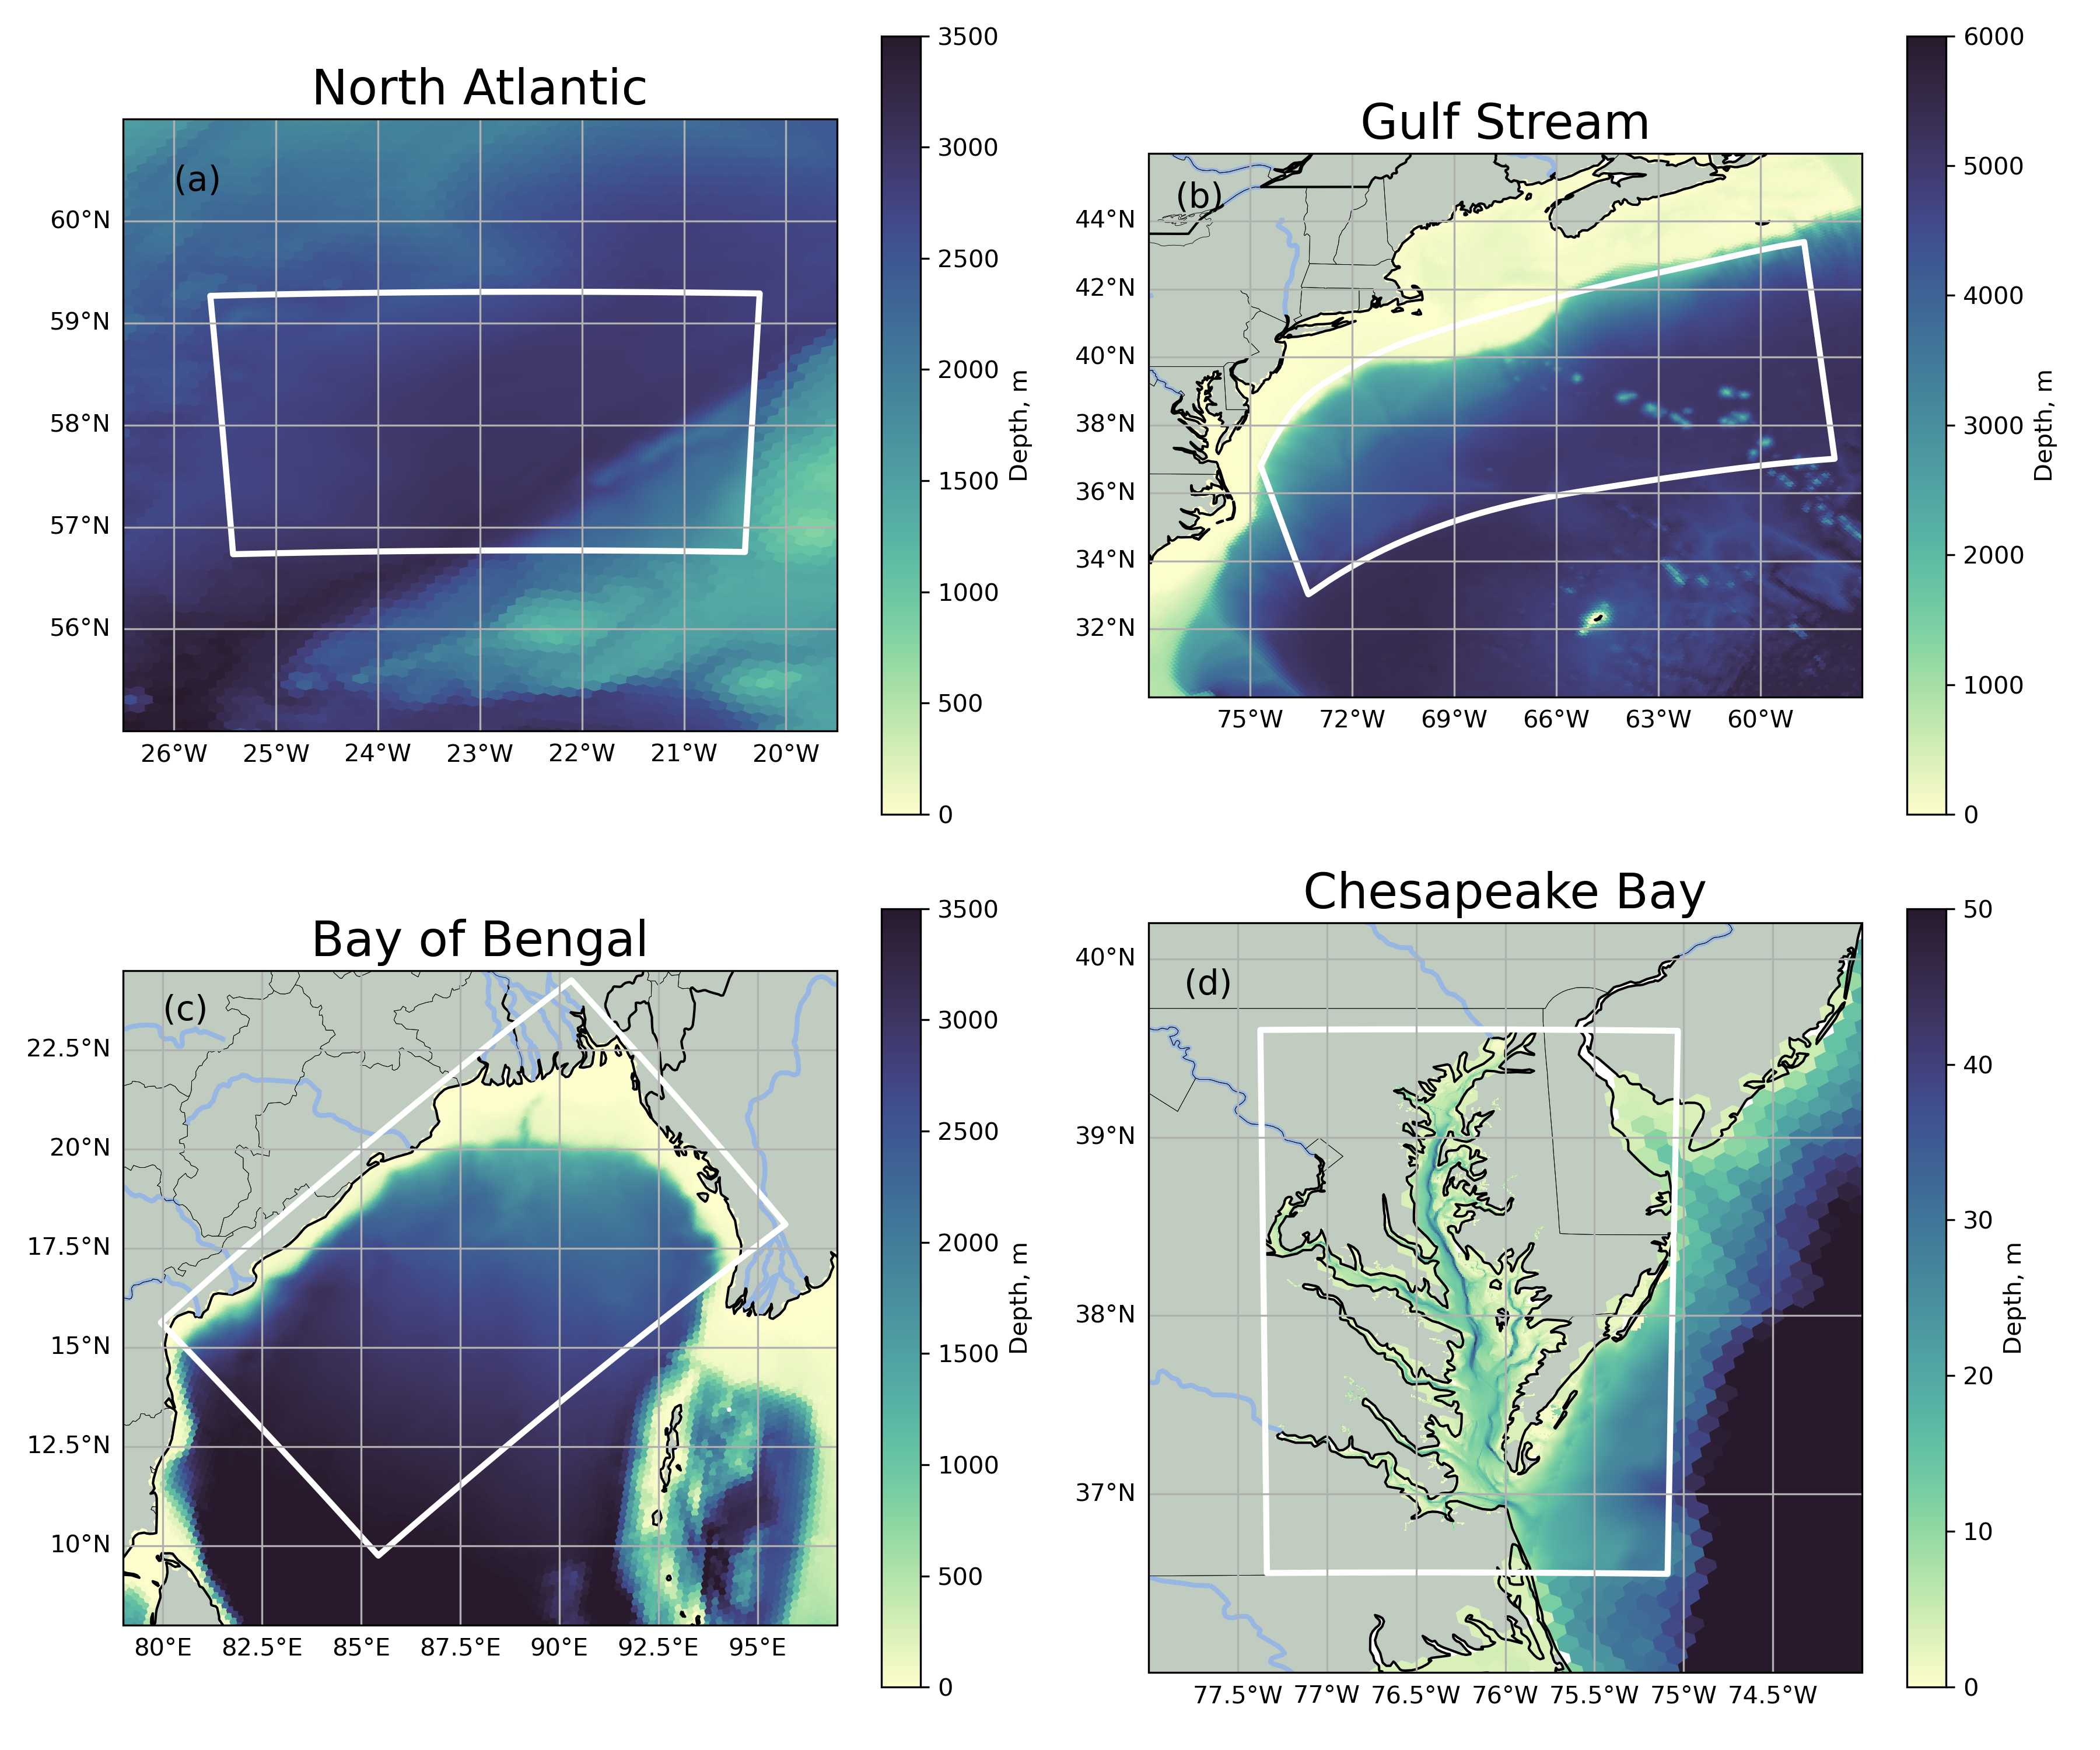
\includegraphics[width=\textwidth]{Figures/model_bathymetries_v20260629.png}
	\caption{Combined \MPAS and \ROMS bathymetries for the four application domains.}
	\label{fig:zed_comparison}
\end{figure}


The experiments reported here use four \ROMS regional domains, ordered so that each introduces a further complication for the transfer: land masks, steep bathymetric gradients, and \ROMS cells progressively smaller than anything the \MPAS mesh resolves. Their characteristic lengths range from \SI{4}{\kilo\metre} to sub-kilometre (\SI{0.6}{\kilo\metre}) estuarine scales.

The first is a North Atlantic implementation of the Near Inertial Shear and Kinetic Energy in the North Atlantic Experiment (NISKINe) model \citep{simmons2024niskine}, designed to study the generation, propagation, and dissipation of near-inertial waves and their interaction with mesoscale and submesoscale structure in the Iceland Basin. Its characteristic length is \SI{2}{\kilo\metre} over water approximately \SI{2750}{\metre} deep and carries no land mask, so it exercises the transfer with neither masking nor sharp topography.

The Gulf Stream domain adds bathymetric relief. Its curvilinear mesh, with a characteristic length of \SI{1.6}{\kilo\metre}, follows the meandering path of the western boundary current, and it also carries no land mask, but including the southern edge of Georges Bank gives it substantially sharper bathymetric gradients than the open-ocean case.
%
The third domain covers most of the Bay of Bengal with a characteristic length of \SI{4}{\kilo\metre} and adds a nearshore setting: land masks on all sides, steep bathymetric gradients, and river inputs drawn from the GloFAS-ERA5 global river discharge reanalysis \citep{harrigan2020glofas}. The fourth is the Chesapeake Bay application developed to study the sensitivity of estuarine hypoxia to external physical forcing \citep{st2024sensitivity}. Its estuarine scales fall well below what the local \MPAS grid represents and much of the domain is masked in \MPAS, so it places the greatest demand on the transfer of the four. Their geographic extent and bathymetric characteristics are shown in Fig.~\ref{fig:zed_comparison}.


\TODOc{Kyle/Rob: Add more background/motivation on \ROMS and how having this downscaling ability can help better understand ocean dynamcis in regions of interest}

%

\FloatBarrier
\section{Methodology}\label{sec:methods}

The global \MPAS model uses Centroidal Voronoi Tesselation (CVT) to generate a variable resolution mesh that provides a smooth coastal to deep-ocean transition region and minimizes diffusive effects during long term termporal integration. However, the regional \ROMS model with typically a higher spatiotemporal resolution uses a curvilinear grid in the radial direction, leading to a regionally structured mesh embedded in an unstructured global polygonal mesh. We will discuss the problem setup, the complication due to variation in axial coordinate systems~\citep{petersen2015evaluation}, and describe the algorithm that achieves consistent embeddings to transfer the forcing conditions accurately and efficiently.

\subsection{Problem statement and notation}\label{sec:problem}

The central design constraint is that the source and target
discretizations differ in \emph{both} the horizontal tessellation
(unstructured Voronoi vs.\ structured curvilinear) \emph{and} the
vertical coordinate (fixed-$z$ vs.\ terrain-following sigma), as
illustrated in Figure~\ref{conv:fig:coord-mismatch}. 


Let the {\MPAS} global ocean mesh cover a region of interest with
$n_M$ Voronoi cells, each carrying a column of tracer values on
$K_M$ fixed depth levels $\{\zmpas_k\}_{k=1}^{K_M}$. Let the \ROMS{}
target grid have $n_R$ horizontal cells, each with a column of
$K_R$ terrain-following (sigma) levels whose absolute depths
$\{\zmpas_\ell^{(i)}\}_{\ell=1}^{K_R}$ depend on the local bathymetry
$H_i$ and free-surface elevation $\zeta_i$ through the Song--Haidvogel
stretching transformation~\citep{song1994semi,shchepetkin2005regional}.
A three-dimensional \MPAS source field is then given by the array
$\Phi \in \mathbb{R}^{n_M \times K_M}$ and the projected \ROMS 
regional target field is $\Psi \in \mathbb{R}^{n_R \times K_R}$. The problem at hand is to compute consistent, and conservative three-dimensional solution transfer from global \MPAS models to the \ROMS model to achieve one-way submesoscale resolving solutions.

Note that a fully
three-dimensional intersection of two such cell complexes is possible, but in general will involve $O(n_M n_R K_M K_R)$ computational complexity to decipher candidate overlaps (worst case),
and can produce multiple sliver polyhedra whose quadratures are ill-conditioned.
We instead exploit the fact that the \MPAS{} vertical coordinate is
horizontally uniform (the depth levels $\zmpas_k$ do not vary between
columns) to factor the transfer into a horizontal remap and a
one-dimensional vertical remap.


\begin{figure}[htbp]
\centering
\begin{subfigure}{0.43\textwidth}
	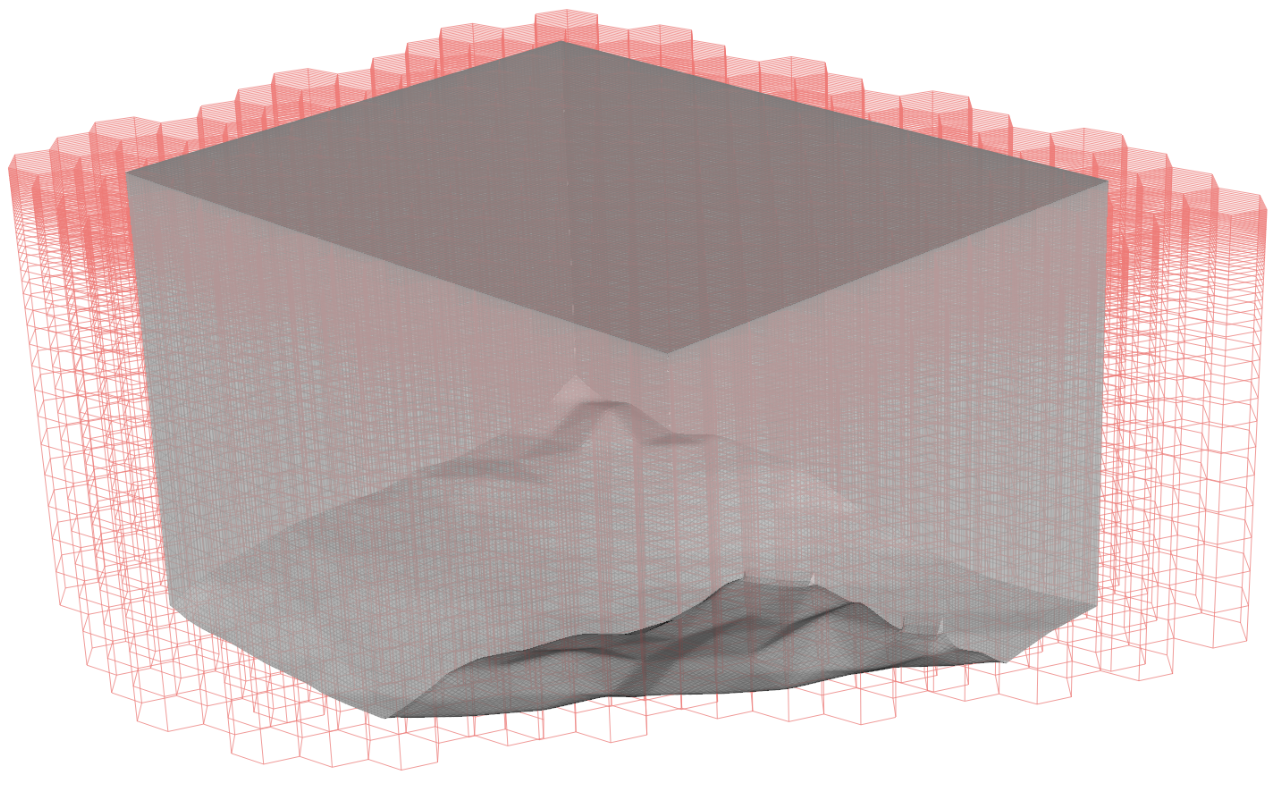
\includegraphics[width=\textwidth]{Figures/conv_embedded_3dmesh.png}
	\caption{Regional \ROMS mesh embedded within the \MPAS source domain.}
	\label{conv:fig:embed3d}
\end{subfigure}\hfill
\begin{subfigure}{0.55\textwidth}
	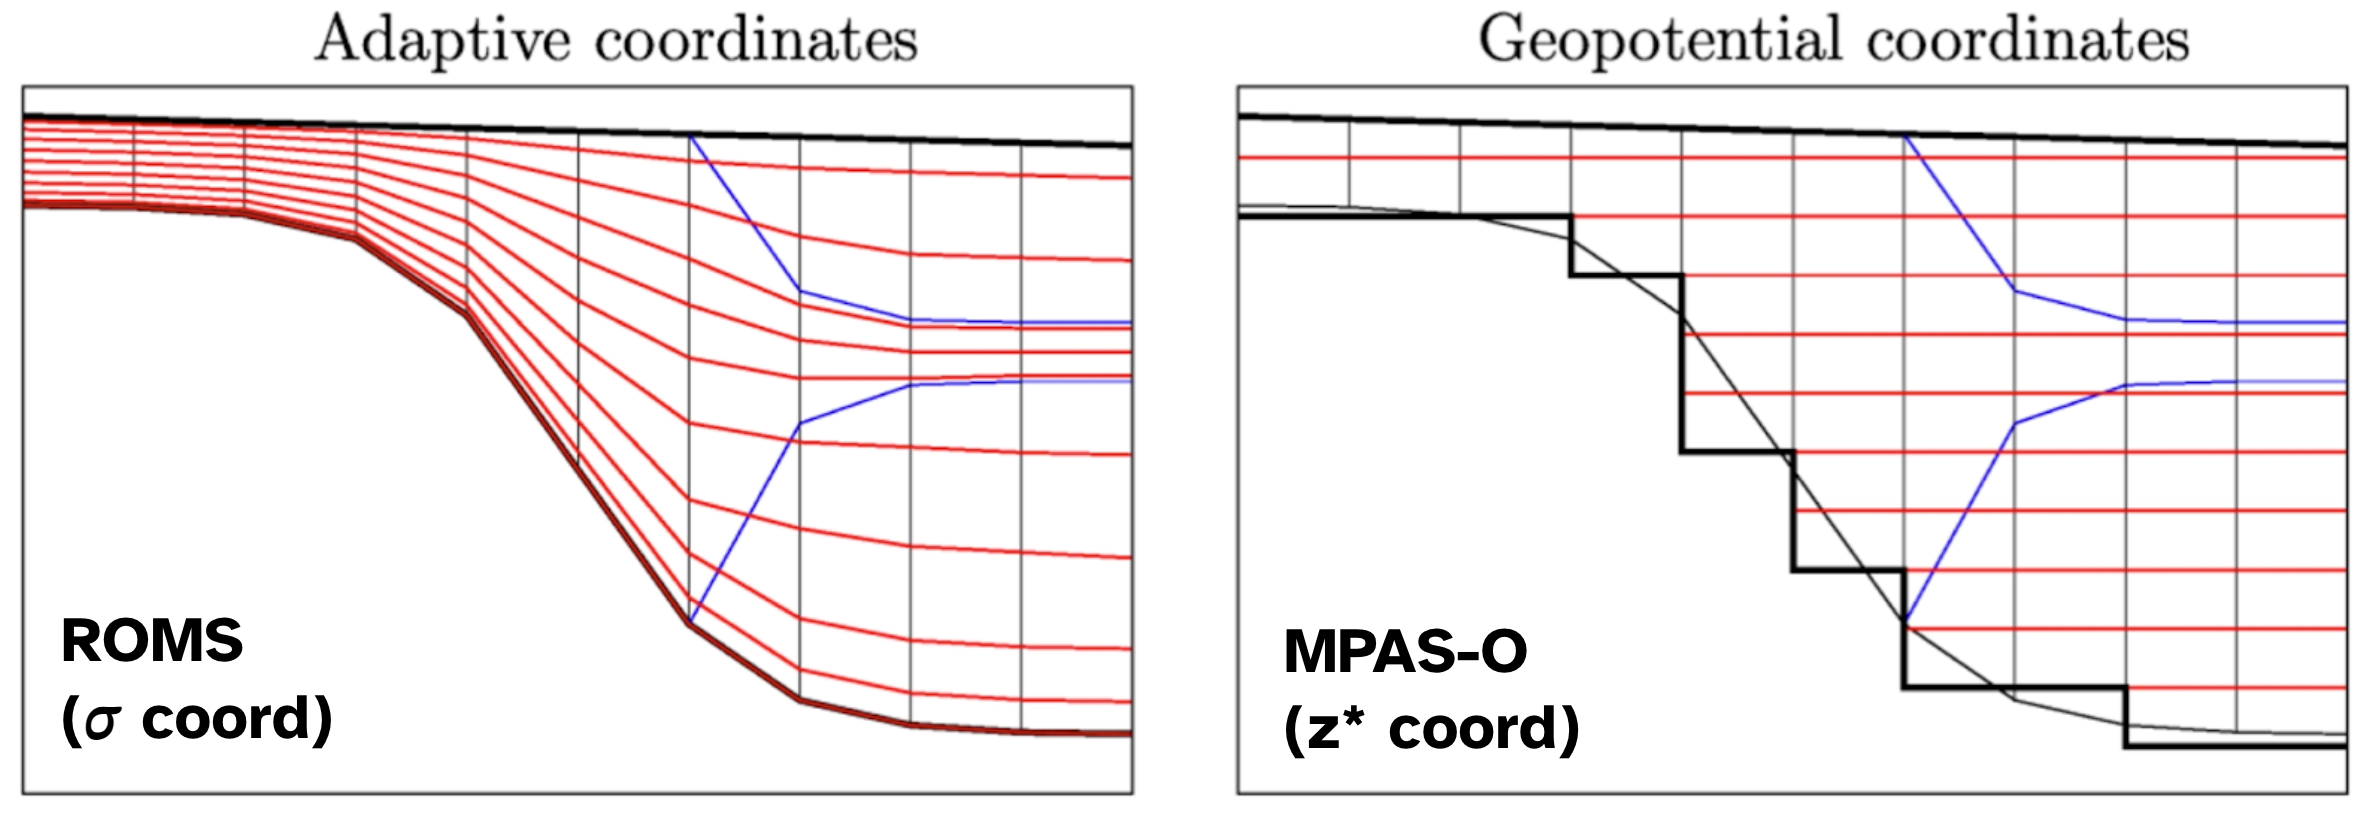
\includegraphics[width=\textwidth]{Figures/conv_zcoord_contrast.png}
	\caption{\ROMS terrain following ($\sigma$) and \MPAS geopotential ($z^*$) coordinates.}
	\label{conv:fig:zcoord}
\end{subfigure}
\caption{Horizontal (left) and vertical (right) discretizations used in the transfer.}
\label{conv:fig:coord-mismatch}
\end{figure}

Throughout the manuscript, we indicate source \MPAS cell indices with the subscript $j$, and target \ROMS cells with the $i$ index, while $k$ and $\ell$ index source and target vertical levels respectively. Uppercase $\Phi,\Xi,\Psi$ denote whole
three-dimensional arrays, and the corresponding lowercase $\phi,\psi$
denote a single horizontal slab extracted at a fixed level, so that
$\phi_j=\Phi_{j,k}$ for the level $k$ under discussion. Cell areas carry the mesh as a superscript: $A^M_j$ is the
area of source cell $j$, $A^R_i$ that of target cell $i$, and $A_{ij}$
the area of their intersection. All geometry is treated on the unit
sphere, areas are spherical areas computed by L'Huilier's excess
formula, and horizontal weights are area-based so that the operators
are independent of the absolute mesh radius.

% Methods section.
\subsection{Separable volumetric remapping}\label{conv:sec:methods}

Writing $\Xi$ for the intermediate field that results from transferring
every source level horizontally, and $\mathcal{V}$ for the column-wise
vertical remap, the composed transfer is
\begin{equation}
  \Xi_{i,k}=\sum_j W_{ij}\Phi_{j,k},\qquad \Psi=\mathcal{V}(\Xi),
  \label{conv:eq:tensor}
\end{equation}

where the horizontal map $W$ is reused unchanged at every source level
and $\mathcal{V}$ acts independently on each target column. This
prism-based 2D$\times$1D construction avoids sliver polyhedra while
retaining the column geometry that the vertical remap requires. The two
factors are developed in turn in \S\ref{sec:horizontal} and
\S\ref{sec:vertical}. A schematic of the volumetric remapping algorithm is shown in Figure~\ref{fig:remap_methods}.


\begin{figure}[htbp]
	\centering
	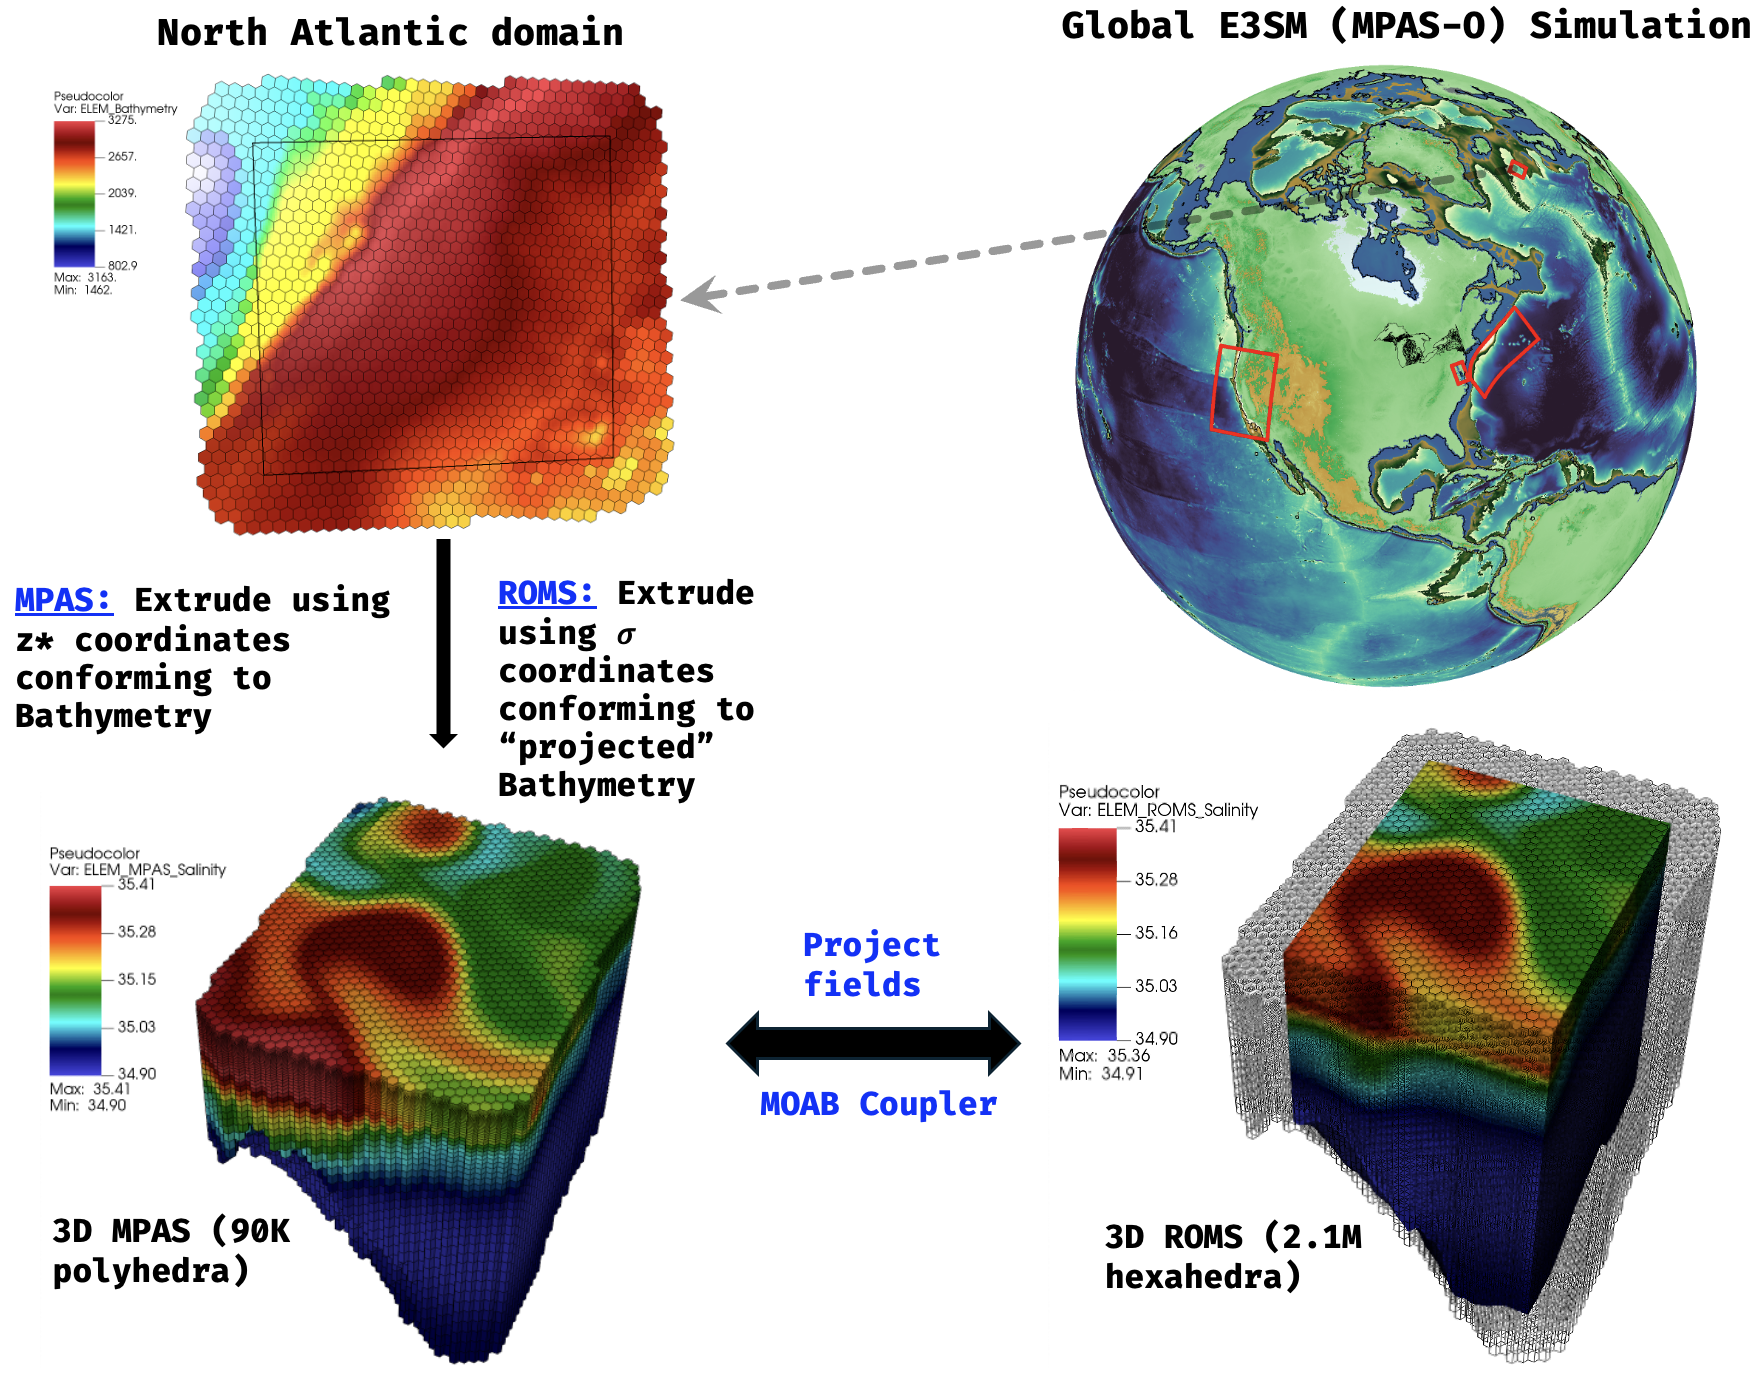
\includegraphics[width=\textwidth]{Figures/remapping_schematics.png}
	\caption{Schematic of the offline volumetric transfer and regional domains.}
	\label{fig:remap_methods}
\end{figure}


\subsection{Horizontal remap as a sparse linear map}\label{sec:horizontal}

There are different remapping choices that one could utilize to take the 2D surface layer from \MPAS and project it to an embedded \ROMS regional domain. The standard approach is to use the $L_2$ minimization that preserves both the global and local integrals of the fields for exact conservation. However, due to the disparity in the resolution between the \MPAS and \ROMS meshes, the coarse-to-fine projections can yield severe mesh imprinting artifacts as demonstrated by experiments on the North-Atlantic domain in Fig.~\ref{fig:mesh-imprinting}. Here, the \MPAS meshes are about \emph{5x} coarser than the \ROMS meshes, which is already yielding severe imprinting, which can cause instability in the \ROMS simulations.

For a fixed source depth level $k$, the horizontal factor $W$ of
Eq.~\eqref{conv:eq:tensor} acts on the level slab
$\phi=\Phi_{:,k} \in \mathbb{R}^{n_M}$ as the sparse linear map
\begin{equation}
	\psi_i \;=\; \sum_{j=1}^{n_M} W_{ij}\, \phi_j ,
	\qquad W \in \mathbb{R}^{n_R \times n_M},
	\label{eq:linear-map}
\end{equation}
in the linear-maps-for-remapping sense
of~\citet{ullrich2015arbitrary,ullrich2016tempestremap}. Two
constructions of the weights in Eq.~\eqref{eq:linear-map} are
considered below, and they differ in whether conservation or
smoothness is enforced.

\paragraph{Conservative finite-volume (FV) map.}
The first-order conservative finite-volume linear-map ~\citep{jones1999scrip} is computed based on the full supermesh in order to account for the contributions from all partial subcell geometry neighbors from the source mesh overlapping the target elements. This sets the
weight to the area of geometric overlap between target cell $i$ and
source cell $j$, normalized by the target area,
\begin{equation}
	W^{\mathrm{FV}}_{ij} \;=\; \frac{|\Omega_i \cap \Omega_j|}{|\Omega_i|}
	\;=\; \frac{A_{ij}}{A^R_i},
	\label{eq:fv-weight}
\end{equation}
where $\Omega_i$, $\Omega_j$ are the (spherical) target and source
polygons and $A_{ij}$ their intersection area. This map is
\emph{conservative only over the target-covered subdomain}, a
qualification that matters here because the \ROMS{} target is a bounded
region embedded in a global \MPAS{} source: because
$\sum_i A_{ij} = A^M_j$ holds only for a source cell fully covered by the
union of target cells, the area-weighted integral identity
$\sum_i A^R_i \psi_i = \sum_j A^M_j \phi_j$ is exact for source cells
interior to the target footprint and is broken for source cells that
the limited-domain target only partially overlaps. Conservation
therefore applies to the covered interior, never to the source cells
straddling the target boundary; this is the boundary qualification we
enforce operationally through the interior/partial classification of
\S\ref{sec:classification}. The map is first-order accurate and, being
a convex average of the source values ($W^{\mathrm{FV}}_{ij}\ge 0$,
$\sum_j W^{\mathrm{FV}}_{ij}=1$ on fully-covered cells), it is
unconditionally monotone.

\paragraph{Normalized bilinear map.}
The bilinear map locates each target-cell centroid within the source
\MPAS triangulation, forms bilinear interpolation weights
$b_{ij}$ from the enclosing source elements, and row-normalizes them, following the linear-map framework of~\citet{ullrich2015arbitrary,ullrich2016tempestremap}.
\begin{equation}
	W^{\mathrm{BL}}_{ij}
	\;=\; \frac{b_{ij}}{\sum_{j'} b_{ij'}} ,
	\label{conv:eq:bilin-weight}
\end{equation}
so that constant fields are reproduced exactly
($\sum_j W^{\mathrm{BL}}_{ij}=1$). The bilinear map is not globally
conservative by construction, since its column sums are not area ratios Equation.~\ref{eq:fv-weight}. It is, however, second-order accurate on smooth fields and, more importantly for the downscaling setup, it does not tie the target values to the piecewise-constant average of a single source cell. The nonnegative weights form a convex combination that preserves the range of contributing source values, so the map is property-preserving. Its second-order horizontal accuracy does not raise the order of the composed transfer, which is limited by the conservative vertical remap of \S\ref{sec:vertical}, as discussed in \S\ref{conv:sec:conv}.



\subsection{Issues with conservative FV map for tracers}\label{sec:why-not-fv}

The conservative finite-volume (FV) map in \eqref{eq:fv-weight} is the lowest-order case of the conservative \(L_2\)-minimization framework used for general mesh remapping \citep{ullrich2015arbitrary,ullrich2016tempestremap}. Given compatible source and target bases, the transferred field minimizes the overlap-domain error
\begin{equation}
	\int_{\Omega}(f-g)^2\,\mathrm{d}\Omega ,
	\label{eq:l2-min}
\end{equation}
leading to a discrete system $W_{S\rightarrow T}G=F$. Higher-order conservative, monotone, and smooth alternatives are available \citep{lauritzen2008monotone,lee1997mba}; here we focus on the first-order FV map and the normalized bilinear map in \eqref{conv:eq:bilin-weight}, which capture the main trade-off relevant to MPAS--ROMS downscaling.

We retain the FV map for coverage classification (\S\ref{sec:classification}), since its overlap-area weights provide a meaningful geometric coverage fraction. We do not use it for tracer transfer, however, because it produces mesh imprinting.

In the configurations considered here the \ROMS cells are typically much smaller than the \MPAS ocean model cells, that is $\hRatio\ll1$. Under first-order FV remapping, all fine target cells lying within a given \MPAS Voronoi cell receive the same source-cell average. The resulting field is therefore piecewise constant on the source tessellation, even though it is represented on the fine ROMS grid. This appears as a staircase pattern whose discontinuities follow MPAS cell edges.

These discontinuities are not physical gradients. They are introduced solely by the transfer operator and can inject grid-scale noise or adjustment features aligned with the source mesh when the field is used to initialize or force a regional model. The problem is especially consequential for fields that should vary smoothly at the regional scale.

The normalized bilinear map removes the leading-order imprint by interpolating continuously across source mesh rather than assigning constant cell averages, at the cost of exact global conservation. For boundary and initial-condition forcing we regard this as an acceptable compromise, since \ROMS evolves its tracer inventory with its own conservative transport scheme, whereas mesh-imprinted forcing introduces artificial gradients that can persist in the interior solution. The argument does not extend to applications that require strict conservation of the horizontally transferred inventory; those would need an additional correction.

The verification metrics reported here, $\Lone$, $\Ltwo$, and $\Linf$ of Eq.~\eqref{conv:eq:norms}, assess pointwise round-trip accuracy rather than the global horizontal inventory error
\begin{equation}
	\left|\sum_i A^R_i\psi_i-\sum_j A^M_j\phi_j\right| .
	\label{eq:inventory-error}
\end{equation}
Vertical conservation, where needed, is provided separately by the operator of \S\ref{sec:vertical} without reintroducing horizontal imprinting.

Figure~\ref{fig:mesh-imprinting} demonstrates the effect using projected bathymetry over the refined North Atlantic domain. The FV result (centre) reproduces the MPAS Voronoi tessellation as piecewise-constant patches with sharp artificial steps, while the normalized bilinear result (right) remains smooth. Bathymetry provides a useful example because it directly affects the ROMS sigma-coordinate geometry; imprinting in the transferred field therefore perturbs the vertical grid as well as the horizontal representation.


\begin{figure}[htbp]
	\centering
	\begin{subfigure}{0.29\textwidth}
		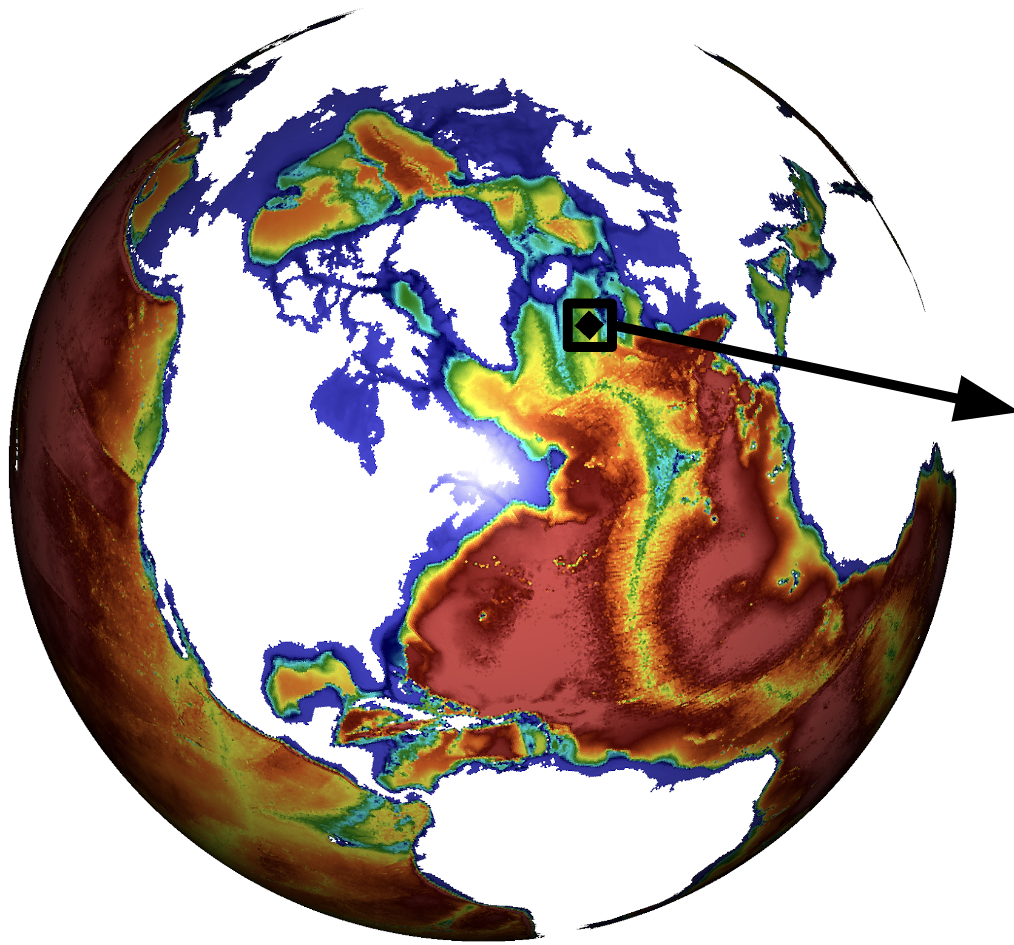
\includegraphics[width=\textwidth]{Figures/fig_regional_refinement.png}
		\caption{Regionally refined domain.}
		\label{fig:imprint-region}
	\end{subfigure}\hfill
	\begin{subfigure}{0.35\textwidth}
		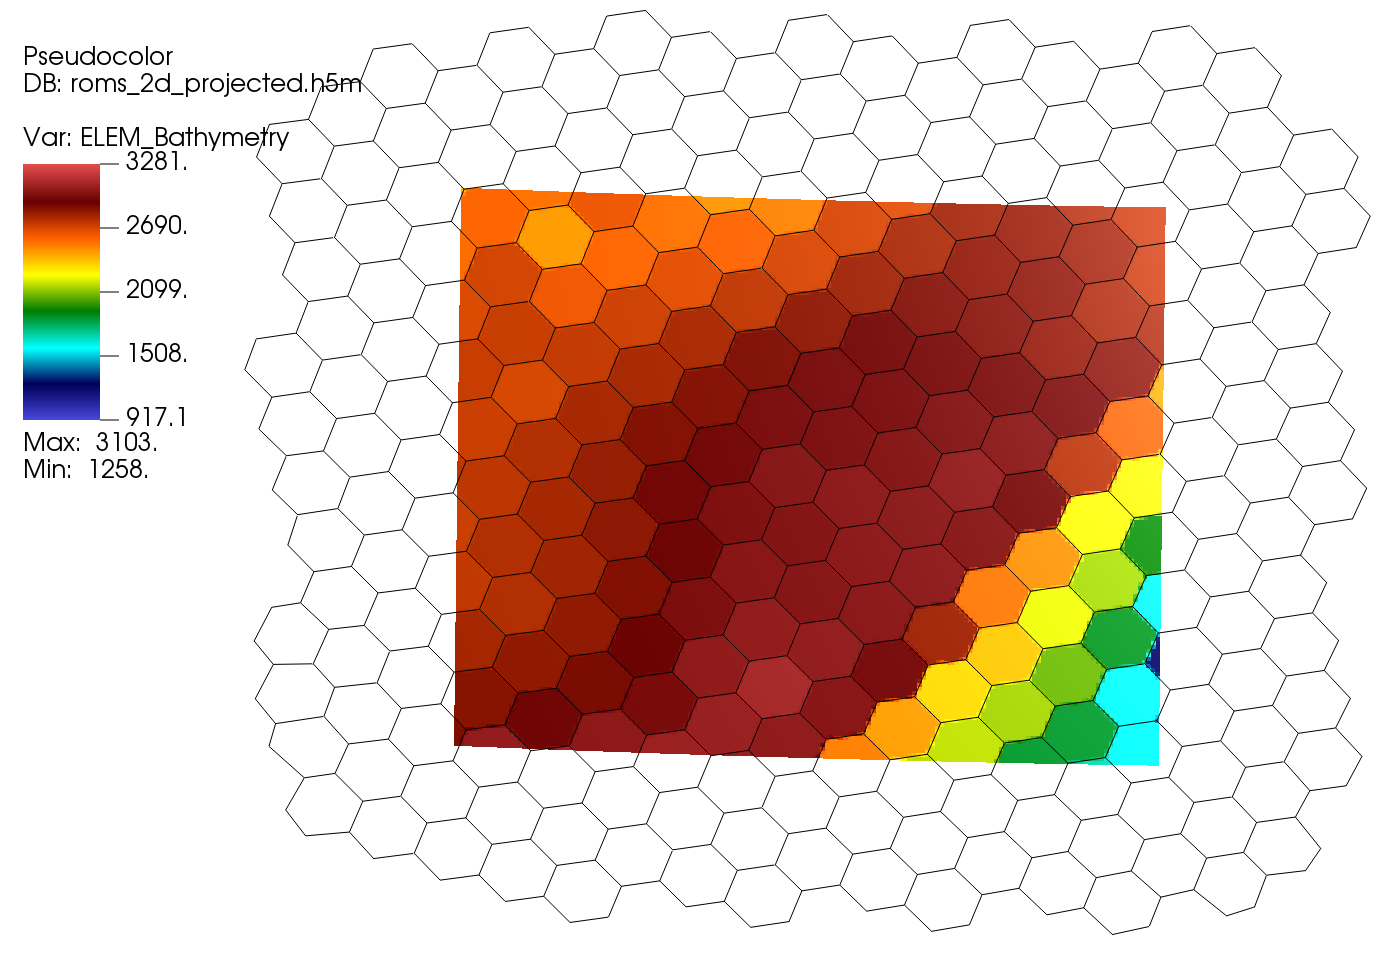
\includegraphics[width=\textwidth]{Figures/conv_bathy_fv.png}
		\caption{Conservative FV ($L_2$-minimizing) map.}
		\label{conv:fig:fv-remap}
	\end{subfigure}\hfill
	\begin{subfigure}{0.35\textwidth}
		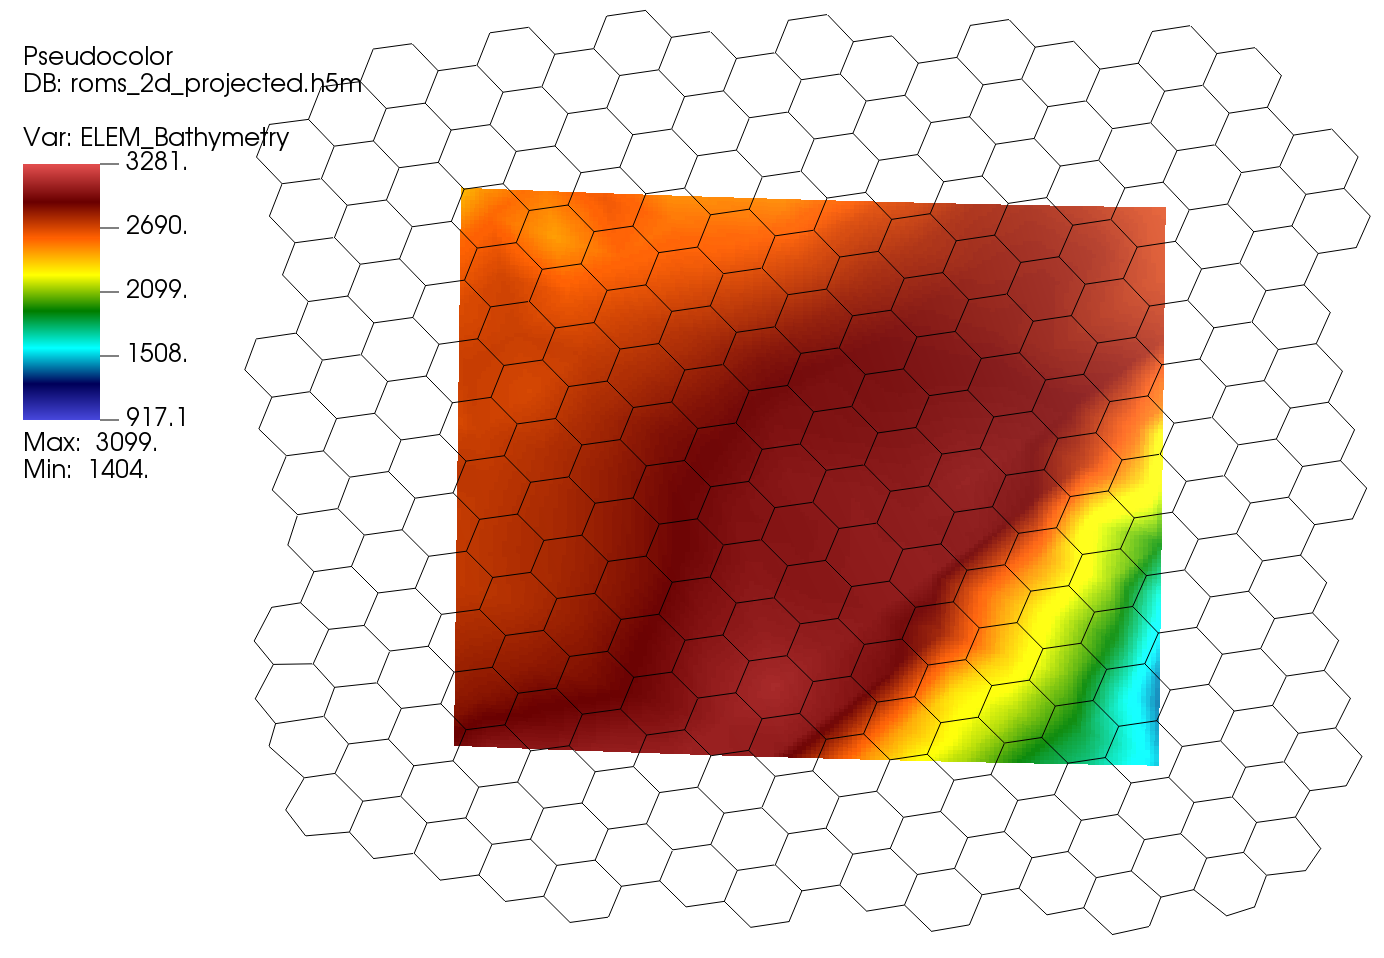
\includegraphics[width=\textwidth]{Figures/conv_bathy_bilinear.png}
		\caption{Bilinear projection.}
		\label{conv:fig:bilinear-remap}
	\end{subfigure}
	\caption{Mesh imprinting in the North Atlantic domain. The conservative FV map reproduces the \MPAS Voronoi tessellation as piecewise-constant patches, whereas the normalized bilinear map remains smooth.}
	\label{fig:mesh-imprinting}
\end{figure}


\subsection{Vertical remap of each column}\label{sec:vertical}

Each intermediate column is assigned physical source depths taken from the nearest source column, and is then remapped onto the local target depths using a monotone, piecewise cubic-Hermite interpolant (PCHIP), where the terrain-following depths follow from the target bathymetry and free-surface ocean elevation (SSH). The property preserved in the vertical direction is the integral of the reconstructed point-sampled profile over each target layer, which for piecewise average degrees-of-freedom originating from finite-volume solvers results in a remap of source-layer averages. Outside the source depth range the profile is held at the nearest endpoint rather than extrapolated for tracer fields, and velocities are maintained at zero.


The linear map is assembled separately for each direction and is independent of level and field. It is important to note that to supply a full level slab, values below the deepest wet source level (\MPAS axial layer masking) are held at the deepest wet value, resembling nearest neighbor extrapolation. The extended tail is discarded when the column is restricted to its physical depth range. This is held true for true tracers, while velocity fields are zeroed out during extrapolation (no flow conditions). The implications of these approaches to handling strong bathymetry variations will be discussed later.


%We should emphasize that these are properties of the two component operators. Neither individually, nor in combination, do they guarantee that the composed three-dimensional transfer conserves volume-integrated quantities or preserves bounds.

It is noted that the zonal and meridional velocities are transferred component-wise as scalar, Earth-relative fields at horizontal cell centers. No rotation to the curvilinear basis, interpolation to polygonal edges, or discrete divergence constraints are imposed in this transfer. The velocity diagnostics presented in this manuscript measure componentwise transport in a fixed basis. Use of consistent mimetic schemes to dynamically transfer vector fields remains outside the present scope of the paper and will be pursued in future work.

\subsection{Regional domains and metrics}\label{conv:sec:regional-methods}


\TODOc{Kyle: Need to add more details about the metrics that we care about in regional domains. Provide details about nudging, and how \ROMS utilizes the time-dependnet forcing conditions to get a consistent view of the global solution}


The solution verification uses the Gulf Stream and Bay of Bengal domains, while regional application validation also include the North Atlantic and Chesapeake Bay. Regional interpretation relies on relative-vorticity maps and surface kinetic-energy time series.

%

\FloatBarrier
\section{Results}\label{sec:results}
The results section is separated in three parts. We first verify the volumetric remapping algorithm, in two stages: a one-dimensional axial refinement study that isolates the vertical operator, followed by a full volumetric convergence study that identifies the \ROMS characteristic length beyond which further refinement stops improving the transferred state. We then measure the computational performance of the implementation, which exploits the tensor product structure through OpenMP thread-level parallelism. Finally, we present one-way coupled \MPAS-\ROMS simulations in open-ocean, coastal, and estuarine domains, and describe the fine-scale structure they develop that the coarse global \MPAS solution does not represent.

% This file is included by main.tex as part of the Results section.
\subsection{Verification of transfer}\label{conv:sec:results-verification}

\subsubsection{Test configuration}\label{conv:sec:verification-method}
The accuracy of the composed projection is assessed with a round trip study~\citep{mahadevan2022mira}. An \MPAS field $\Phi$ is transferred forward as $\Psi=\mathcal{V}_{M\to R}(W_{M\to R}\Phi)$ and then returned as $\tilde{\Phi}=\mathcal{V}_{R\to M}(W_{R\to M}\Psi)$. We measure the round-trip error $e_{jk}=\tilde{\Phi}_{jk}-\Phi_{jk}$, which lives on the \MPAS mesh, using volume-weighted $L_1$ and $L_2$ norms and an unweighted $L_\infty$ norm:
\begin{align}
  \Lone &= \frac{\sum_{j\in\mathcal{I},k} A^M_j\,\Delta \zmpas_{jk}\,|e_{jk}|}{\sum_{j\in\mathcal{I},k} A^M_j\,\Delta \zmpas_{jk}},\qquad
  \Ltwo = \left(\frac{\sum_{j\in\mathcal{I},k} A^M_j\,\Delta \zmpas_{jk}\,e_{jk}^2}{\sum_{j\in\mathcal{I},k} A^M_j\,\Delta \zmpas_{jk}}\right)^{1/2},\\
  \Linf &= \max_{j\in\mathcal{I},k}|e_{jk}|,
  \label{conv:eq:norms}
\end{align}
where $\Delta \zmpas_{jk}$ is the thickness of level $k$ in \MPAS column $j$, so that $A^M_j\,\Delta \zmpas_{jk}$ is the cell volume, and $\mathcal{I}$ denotes the set of \MPAS cells with complete horizontal coverage in the sense of the classification below. Partial cells, and columns without a valid vertical reconstruction, are excluded, so the three-dimensional support on which the norms are evaluated varies somewhat as the \ROMS mesh is refined. The round trip characterizes the composed operator and does not bound the one-way forcing error, which is the quantity of interest when the transfer is used to drive a regional simulation.

The smooth field used throughout the convergence study is the tensor-product sinusoid
\begin{equation}
 R(\lambda,\varphi,z)=\sin\!\left(\frac{m_\lambda\pi(\lambda-\lambda_0)}{L_\lambda}\right)
 \sin\!\left(\frac{m_\varphi\pi(\varphi-\varphi_0)}{L_\varphi}\right)
 \sin\!\left(\frac{m_z\pi|z|}{H_0}\right),
 \label{conv:eq:analytic}
\end{equation}
where $\lambda$ and $\varphi$ are longitude and latitude, $(\lambda_0,\varphi_0)$ is the southwest corner of the \ROMS bounding box, $L_\lambda$ and $L_\varphi$ are its angular extents, and $(m_\lambda,m_\varphi,m_z)$ are the mode numbers in the two horizontal directions and the vertical. The field has unit amplitude, $(m_\lambda,m_\varphi,m_z)=(2,2,1)$, and $H_0=\SI{4000}{\metre}$. It is transferred alongside salinity, temperature, and the two velocity components from one daily-mean \MPAS state. With $m_z=1$, Eq.~\eqref{conv:eq:analytic} carries only a half wavelength over the full depth, so it is smooth in the vertical by construction. %Sharp features such as the halocline, which the $L_\infty$ diagnostics below implicate, are therefore not represented in the analytic test.

Writing $A_{\mathrm{bbox}}$ for the area of the common bounding box, $n_{\mathrm{bbox}}$ for the number of \MPAS cells whose centers fall inside it, and $n_{\mathrm{cells}}$ for the number of \ROMS cells, the characteristic lengths of the two meshes are $\hM=\sqrt{A_{\mathrm{bbox}}/n_{\mathrm{bbox}}}$ and $\hR=\sqrt{A_{\mathrm{bbox}}/n_{\mathrm{cells}}}$, and their ratio is $\hRatio=\hR/\hM$. Four nested \ROMS meshes, r1 (coarsest) through r4 (finest), are used in each region. Their inventory is given in Table~\ref{conv:tab:grid-inventory}.

\begin{table}[htbp]
\centering
\small
\setlength{\tabcolsep}{3pt}
\caption{\ROMS mesh inventory, r1 (coarsest) to r4 (finest).}
\label{conv:tab:grid-inventory}
\begin{tabular}{llrrrr}
\toprule
Region & Label & $\eta_\rho\times\xi_\rho$ & Cells$^{\dagger}$ & $\hR$ (km) & $\hRatio$ \\
\midrule
\multirow{4}{*}{Gulf Stream} & r1 & $38\times112$ & $4107$ & $20.07$ & $2.12$ \\
& r2 & $114\times334$ & $37629$ & $6.70$ & $0.71$ \\
& r3 & $341\times1001$ & $340000$ & $2.24$ & $0.24$ \\
& r4 & $1023\times3003$ & $3068044$ & $0.75$ & $0.08$ \\
\midrule
\multirow{4}{*}{Bay of Bengal} & r1 & $24\times40$ & $897$ & $52.61$ & $3.21$ \\
& r2 & $74\times120$ & $8687$ & $17.45$ & $1.06$ \\
& r3 & $222\times362$ & $79781$ & $5.82$ & $0.35$ \\
& r4 & $666\times1086$ & $721525$ & $1.94$ & $0.12$ \\
\bottomrule
\end{tabular}

\vspace{0.3em}
{\footnotesize $^{\dagger}$Cell counts are $(\eta_\rho-1)(\xi_\rho-1)$, since $\eta_\rho$ and $\xi_\rho$ count \ROMS grid nodes and the transfer operates on the cells they bound.}
\end{table}

The Gulf Stream \MPAS mesh is locally refined to a characteristic length of $\hM=\SI{9.48}{\kilo\metre}$, whereas the coarser Bay of Bengal \MPAS mesh gives $\hM=\SI{16.41}{\kilo\metre}$. The same labels therefore denote different absolute characteristic lengths but comparable relative refinement.


%\paragraph{Coverage classification.}
\label{sec:classification}
Note that the \ROMS mesh is a bounded region embedded in the global \MPAS mesh, so every \ROMS cell is labeled based on whether it is within the convex hull of the \MPAS coverage mesh~\citep{mahadevan2020coupling}. Let $f^M_j$ and $f^R_i$ denote the covered fractions of \MPAS cell $j$ and \ROMS cell $i$, obtained from the overlap areas $A_{ij}$ of the FV supermesh. Cells with $f=1$ are \emph{interior}, and those with $0<f<1$ are only \emph{partially} covered. The interior set, written as $\mathcal{I}$, is the support on which the error norms of \S\ref{conv:sec:verification-method} are evaluated. 

%Coverage-weighted conservation is a separate map property and condition:
%\begin{equation}
%	\sum_i A^R_i f^R_i\,\Xi_{i,k}
%	=\sum_j A^M_j f^M_j\,\Phi_{j,k}.
%	\label{conv:eq:bilin-conservation}
%\end{equation}
%Equation~\eqref{conv:eq:bilin-conservation} is weighted by the covered fractions on both sides, so it constrains only the shared support of the two meshes. It is satisfied by the conservative FV map of Eq.~\eqref{eq:fv-weight} but not by the normalized bilinear map of Eq.~\eqref{conv:eq:bilin-weight}, which is the trade discussed in \S\ref{sec:why-not-fv}.

%The horizontal classification is essentially fixed across each refinement sequence, because it depends on the target footprint rather than on the target spacing. In the Gulf Stream, 10{,}158--10{,}162 source cells are interior and 534--536 are partial across r1--r4, and in the Bay of Bengal, 4249--4265 are interior and 280--320 partial. What does change with refinement is the number of target columns discarded for lack of a valid vertical reconstruction, which is reported alongside the Bay of Bengal sequence below.

\subsubsection{One-dimensional axial refinement study}\label{conv:sec:axial-refinement}

Figure~\ref{conv:fig:physical-1d-workflow} isolates the axial factor under joint refinement of the \MPAS and \ROMS layers. It is a reduced representation of the geometry in Fig.~\ref{conv:fig:coord-mismatch} where the selected nonuniform \MPAS columns retain the physical $z^*$ layer-thickness patterns of the Gulf Stream and Bay of Bengal \MPAS meshes, while the \ROMS layer interfaces are regenerated from the same terrain-following stretching families used by the regional grids. The matching and fixed-bottom extrapolation cases respectively represent a \ROMS column embedded in the resolved \MPAS column [SSH, Bathymetry] range, and a \ROMS column extending slightly beyond it due to the stair stepping of the bathymetry on the finer \ROMS cells. Thus the one-dimensional sequence retains the vertical-coordinate mismatch, and refinement mechanism of the regional cases while removing influence of horizontal remap effects.

The two axial operators are compared here because they sit at opposite ends of the same trade. The conservative axial projection, which is the one used for the three-dimensional transfers reported in this manuscript, reproduces each \ROMS layer integral and is first order in the layer thickness. The PCHIP point projection instead reproduces the profile itself, so it attains higher order on smooth data, but it does not conserve. Over the tested physical columns and the smooth sinusoidal profile, the conservative projection converges at first order, consistent with the $\mathcal{O}(h)$ reference drawn in the figure, while the point projection converges faster. The two have distinct output semantics, the former evaluated from \ROMS layer integral residuals and the latter as a point-value projection of average values, so the comparison is between the two workflow contracts rather than between interchangeable discrete $L_2$ measures. It is also limited to the physical columns, stretching families, profile, and refinement range tested here.

\begin{figure}[htbp]
\centering
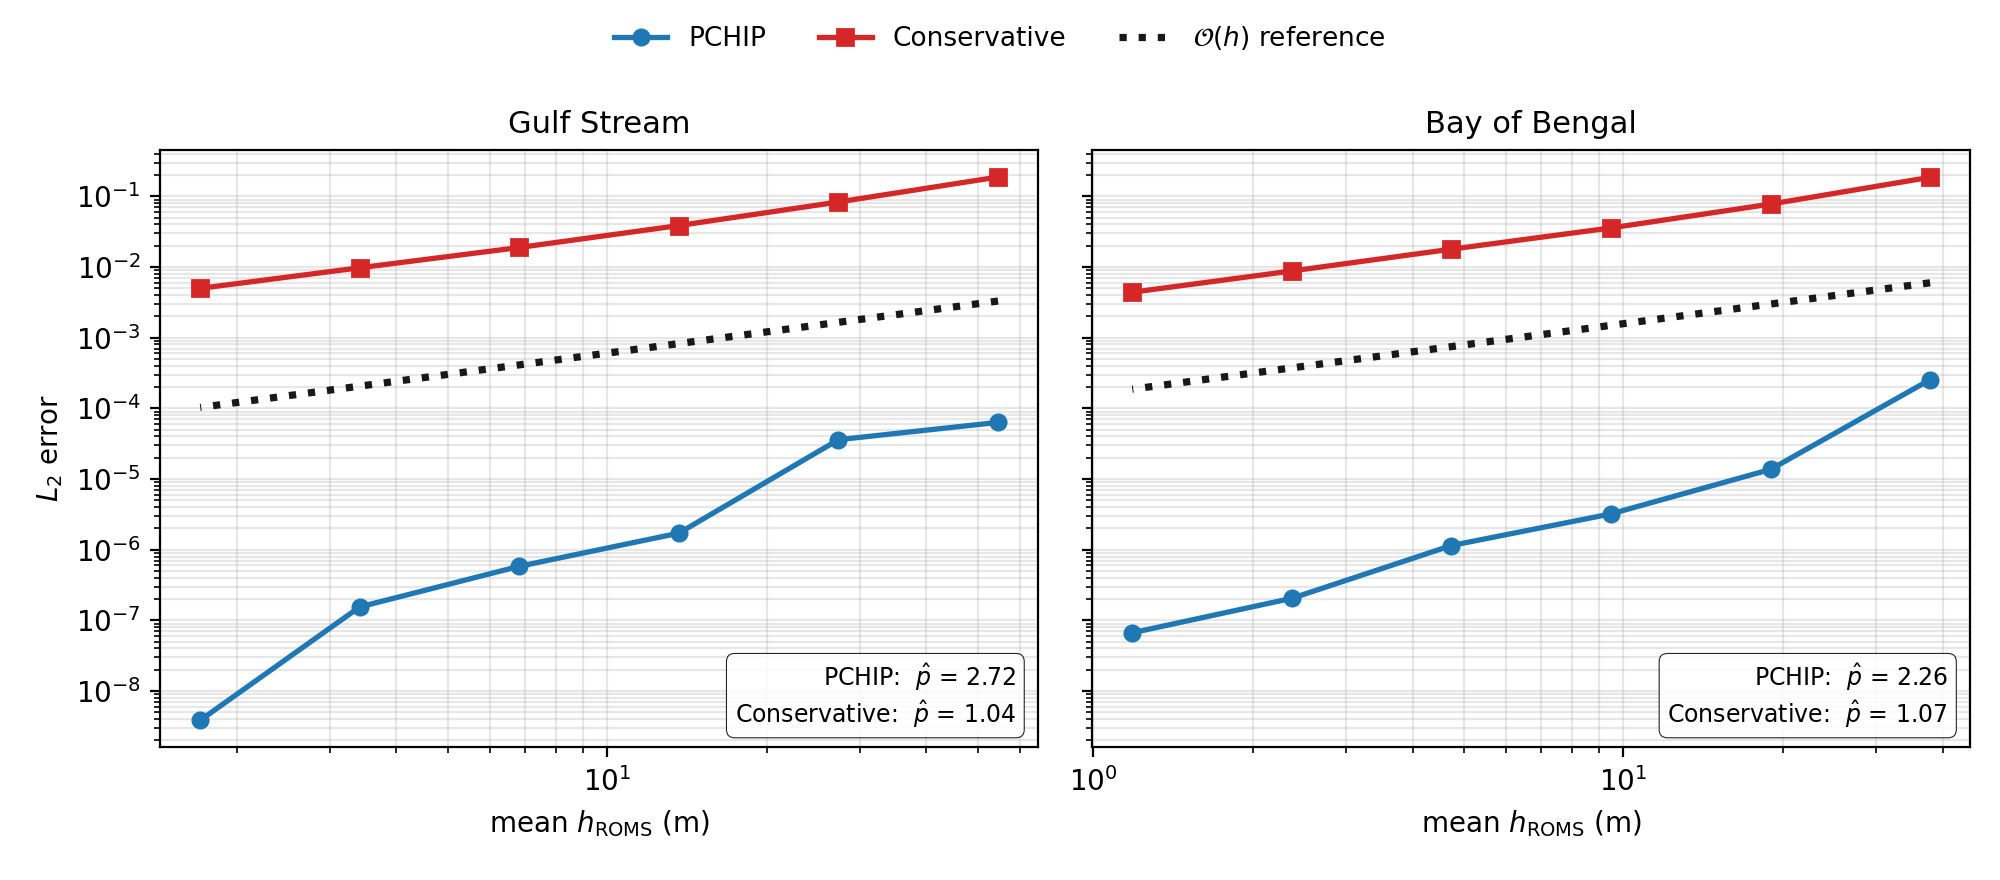
\includegraphics[width=\textwidth]{Figures/conv_1d_convergence.png}
\caption{One-dimensional convergence of the two axial operators. Dotted line: $\mathcal{O}(h)$ reference.}
\label{conv:fig:physical-1d-workflow}
\end{figure}

For the separable transfer in Eq.~\eqref{conv:eq:tensor}, the combined error may be written schematically as
\begin{equation}
  E_{3D}\lesssim C_h h_h^{p_h}+C_z h_z^{p_z}.
  \label{conv:eq:tensor-order}
\end{equation}
When horizontal and axial resolutions are jointly refined at comparable rates, the lower directional observed order in Eq.~\eqref{conv:eq:tensor-order} limits the asymptotic rate of the tensor-product workflow. Thus the observed axial first-order behavior supplies the relevant $\mathcal{O}(h)$ reference for the tested joint refinement. The one-dimensional experiment measures the axial factor only, and it does not independently establish a complete three-dimensional rate or a universal order for every field, mesh, or limiter state.

\subsubsection{Convergence and quantification of error sources}\label{conv:sec:conv}

A convergence study in the usual sense would refine both the \MPAS and \ROMS meshes together. Here the \MPAS global mesh is fixed, as it would be in practice, and we refine only the embedded \ROMS meshes. The sequences below therefore measure how the transfer responds to \ROMS refinement against a fixed \MPAS mesh, not the asymptotic order of the operator.

Figures~\ref{conv:fig:gs-convergence} and~\ref{conv:fig:bob-convergence} show the interior round-trip norms of Eq.~\eqref{conv:eq:norms} versus $\hRatio$ for the two regions. Each panel set reports the volume-weighted $\Lone$ and $\Ltwo$ and the unweighted $\Linf$ for salinity, temperature, the two velocity components, and the smooth analytic field, with scalar errors normalized by representative absolute field magnitudes. Recall from Table~\ref{conv:tab:grid-inventory} that $\hRatio=1$ corresponds to an \MPAS characteristic length of $\SI{9.5}{\kilo\metre}$ in the Gulf Stream and $\SI{16.4}{\kilo\metre}$ in the Bay of Bengal.

%% Gulfstream convergence
\begin{figure}[htbp]
\centering
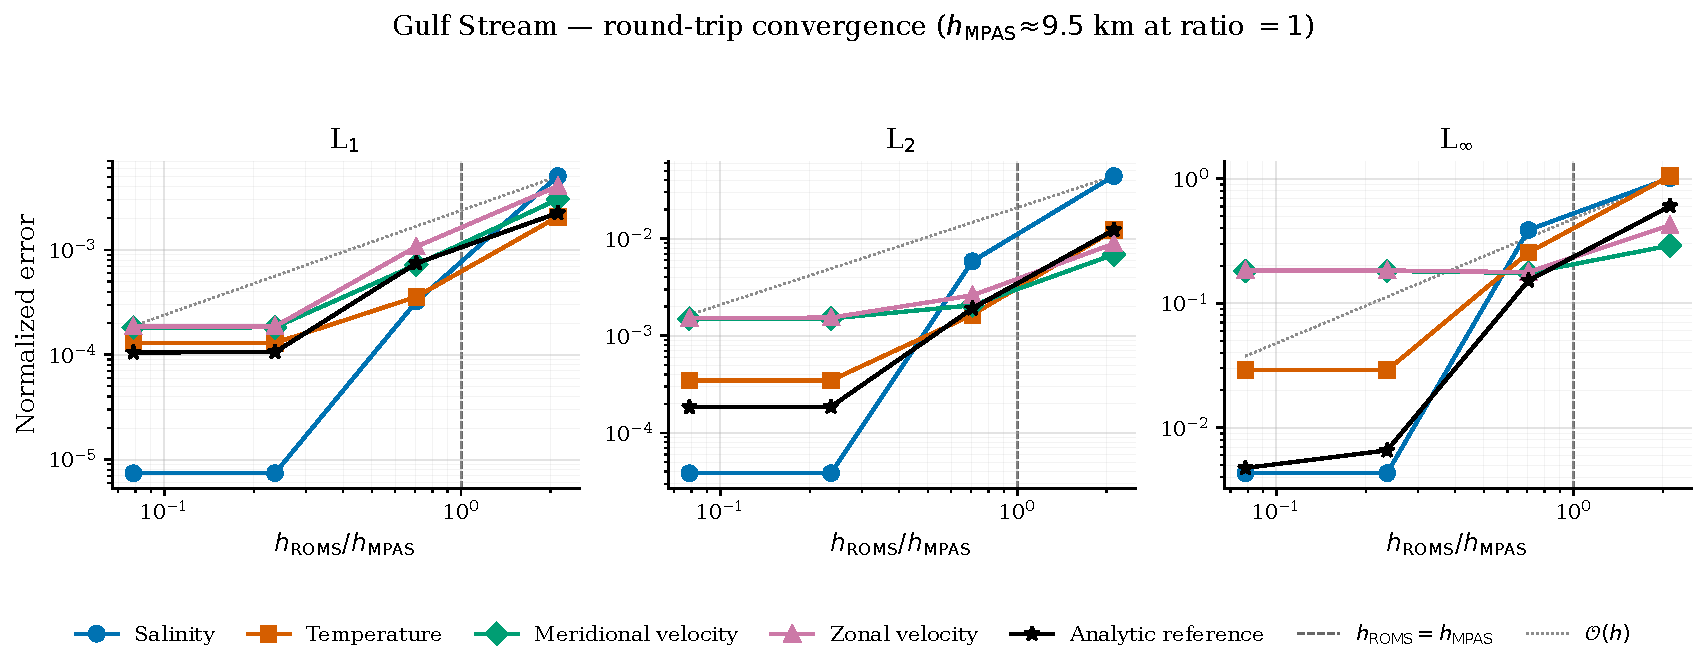
\includegraphics[width=\textwidth]{Figures/conv_convergence_gulfstream.pdf}
\caption{Gulf Stream round-trip errors versus $\hRatio$: $\Lone$ (left), $\Ltwo$ (middle), $\Linf$ (right).}
\label{conv:fig:gs-convergence}
\end{figure}

%% BoB convergence
\begin{figure}[htbp]
\centering
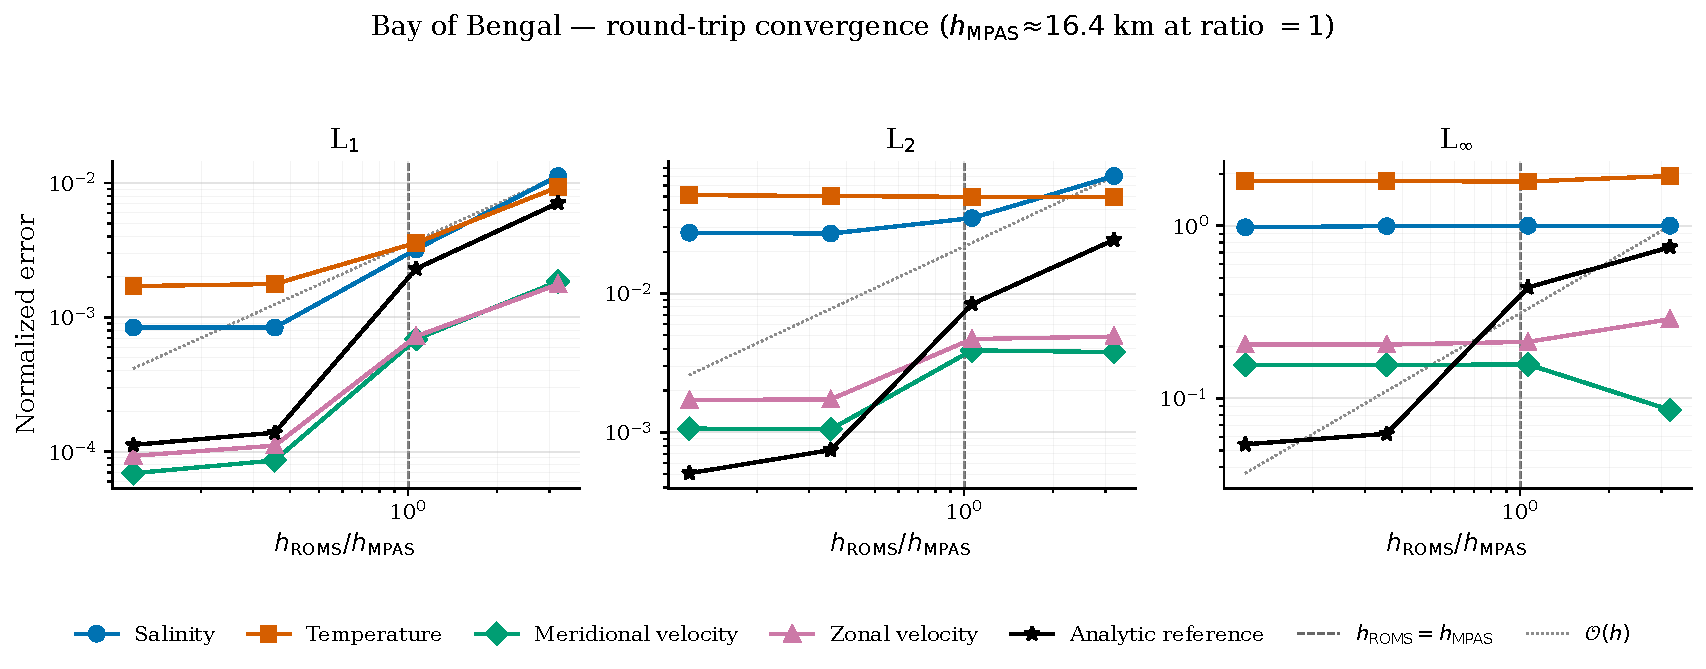
\includegraphics[width=\textwidth]{Figures/conv_convergence_bob.pdf}
\caption{Bay of Bengal round-trip errors versus $\hRatio$: $\Lone$ (left), $\Ltwo$ (middle), $\Linf$ (right).}
\label{conv:fig:bob-convergence}
\end{figure}
\FloatBarrier

Errors decrease over the coarse portion of both sequences, but the real-field errors do not show consistent changes beyond r3 i.e., error plateaus.
%
%The Bay of Bengal r3--r4 comparison deserves particular caution before that plateau is read as a property of the transfer. The number of target columns discarded for lack of a valid vertical reconstruction rises from 18,309 to 166,770 between the two grids, which is 23.0\% and 23.1\% of the respective target cell counts. The discarded region therefore occupies a nearly constant share of the domain, so refinement is not progressively excluding more of it, but that region is resolved differently on the two grids and the norms are evaluated on correspondingly different supports even though the real-field $\Lone$ and $\Ltwo$ values differ by only a few percent. The Gulf Stream sequence discards no columns on any grid, which is consistent with its lack of a land mask and its uniformly deep bathymetry, and it is one reason the two regions should not be compared directly on these norms. A common-support comparison on the finest Bay of Bengal pair would settle whether the plateau is genuine, and we have not run one.
%
Subject to that caveat, the error convergence sequences suggest that $\hRatio\approx0.2$, roughly a fivefold refinement of the \ROMS mesh, is a useful starting point when choosing the \ROMS mesh, and targets at or below $\hRatio\approx0.1$ should be justified by a refinement study for domain of interest when balancing accuracy and computational efficiency. The same value emerges in both an open-ocean and a coastal domain, which is why we offer it as a starting point, but it rests on two domains sharing one \MPAS mesh and a single daily-mean state, so we would recommend confirming it with a short refinement sequence in each new domain rather than adopting it outright.

More generally, for a fixed global \MPAS mesh, a short convergence sequence like this is practical to identify the characteristic length beyond which further refinement of the \ROMS mesh ceases to be worthwhile. As in any multiscale configuration, the lateral boundary conditions supplied from \MPAS carry coarse scale errors that cannot be resolved by \ROMS, or by the forcing itself, as these do not diminish as the \ROMS mesh is refined, so that relative to $\hRatio$ the errors remain $\mathcal{O}(1)$. Because that floor is set by the \MPAS state rather than by the transfer, refining past the point where the sequence flattens buys little in the fidelity of the transferred fields, though we have not measured what it does to the regional solution that evolves from them. The cost, meanwhile, continues to grow: the number of \ROMS cells scales as $\hRatio^{-2}$ and a CFL-limited time step shrinks in proportion to the characteristic length, so integrating a fixed period becomes roughly $\hRatio^{-3}$ more expensive. Choosing the \ROMS characteristic length near the flattening point therefore captures most of the accuracy that the \MPAS state makes available, at a small fraction of the cost of the finest grids tested here. We did not run targets below $\hRatio\approx0.08$, so this is an argument about the range examined rather than an asymptotic claim.

The convergence order of the composed scheme is determined by the rate of the horizontal and vertical components. Imposing conservation on the vertical operator such that each \ROMS layer integral in the reconstructed profile matches the contributions from the \MPAS geopotential coordinate topology, the vertical projection operator mimics a traditional $L_2$ minimization in one dimension, resulting in a first order approximation in the layer thickness. Since the tensor product in Eq.~\eqref{conv:eq:tensor} is no more accurate than its least accurate factor, the composed three-dimensional transfer is first order overall, irrespective of the formal accuracy of the horizontal map. The measured decrease over the convergent portion of both sequences is consistent with this expectation, although four grids are too few to fit an asymptotic rate.

Relaxing the conservation constraint admits alternatives, and this choice is an application decision rather than a purely numerical one. A quasi-interpolant that reproduces the profile rather than its layer integrals reaches higher order on smooth fields, as the one-dimensional comparison of \S\ref{conv:sec:axial-refinement} shows, but forfeits exact conservation, monotonicity, or both depending on how it is constructed. Higher order bought by violating monotonicity can introduce spurious extrema in sharp features such as the thermocline, and a scheme that sacrifices conservation is poorly suited to long integrations where tracer inventories must be maintained. For boundary and initial-condition forcing of a regional model that carries its own conservative transport, either trade may be defensible, and we chose conservation.
%
%\subsubsection{Separating target refinement from the parent representation}\label{conv:sec:controlled}
%
%Because the round trip chains the forward and reverse horizontal maps with the forward and reverse vertical remaps, it cannot by itself indicate which stage limits the result. We did not decompose the operator into horizontal-only and vertical-only legs, which is what would attribute the floor to a specific stage. What the controlled experiments below do instead is hold the \MPAS source fixed while refining only the \ROMS target, which separates the effect of target spacing from the effect of the parent representation without isolating either map. A constant field carried forward and back through the horizontal map alone is reproduced to roundoff, as required by the normalization in Eq.~\eqref{conv:eq:bilin-weight}. In the tensor product split, the composed one-way error, measured against the analytic solution sampled on the target grid, then varies by about 4\% in the Gulf Stream and 5\% in the Bay of Bengal across the whole r1--r4 sequence, which is what we expect when the fixed parent representation, rather than the target spacing, sets the achievable accuracy. The round trip over the same sequence falls by roughly a factor of 23 and 30 respectively, since errors incurred on the forward leg can be undone on the reverse leg, so the round trip is not the one-way error plus a correction, and the two should not be compared directly. These statements apply to the controlled analytic configuration and do not settle the real-field r3--r4 common-support caveat.
%
%Errors grow with depth, and the salinity floors in the two regions differ by about two orders of magnitude. We cannot attribute that gap: the two regions differ in source resolution, in coastal gradient strength, and in the extent of their land masks, and the round-trip metric does not separate these. The persistent $L_\infty$ salinity errors are localized near the surface and near coastlines, and their location shifts with refinement, which is consistent with under-resolved near-surface stratification but does not establish it.


%\FloatBarrier
%\subsection{Performance}\label{conv:sec:performance}
%The benchmark projects four fields from a source mesh of $5.7\times10^6$ polyhedra to a target mesh of $8\times10^6$ elements on one Perlmutter CPU node, using 1--64 OpenMP threads and $N_z=50$ and 100.
%
%\begin{figure}[htbp]
%\centering
%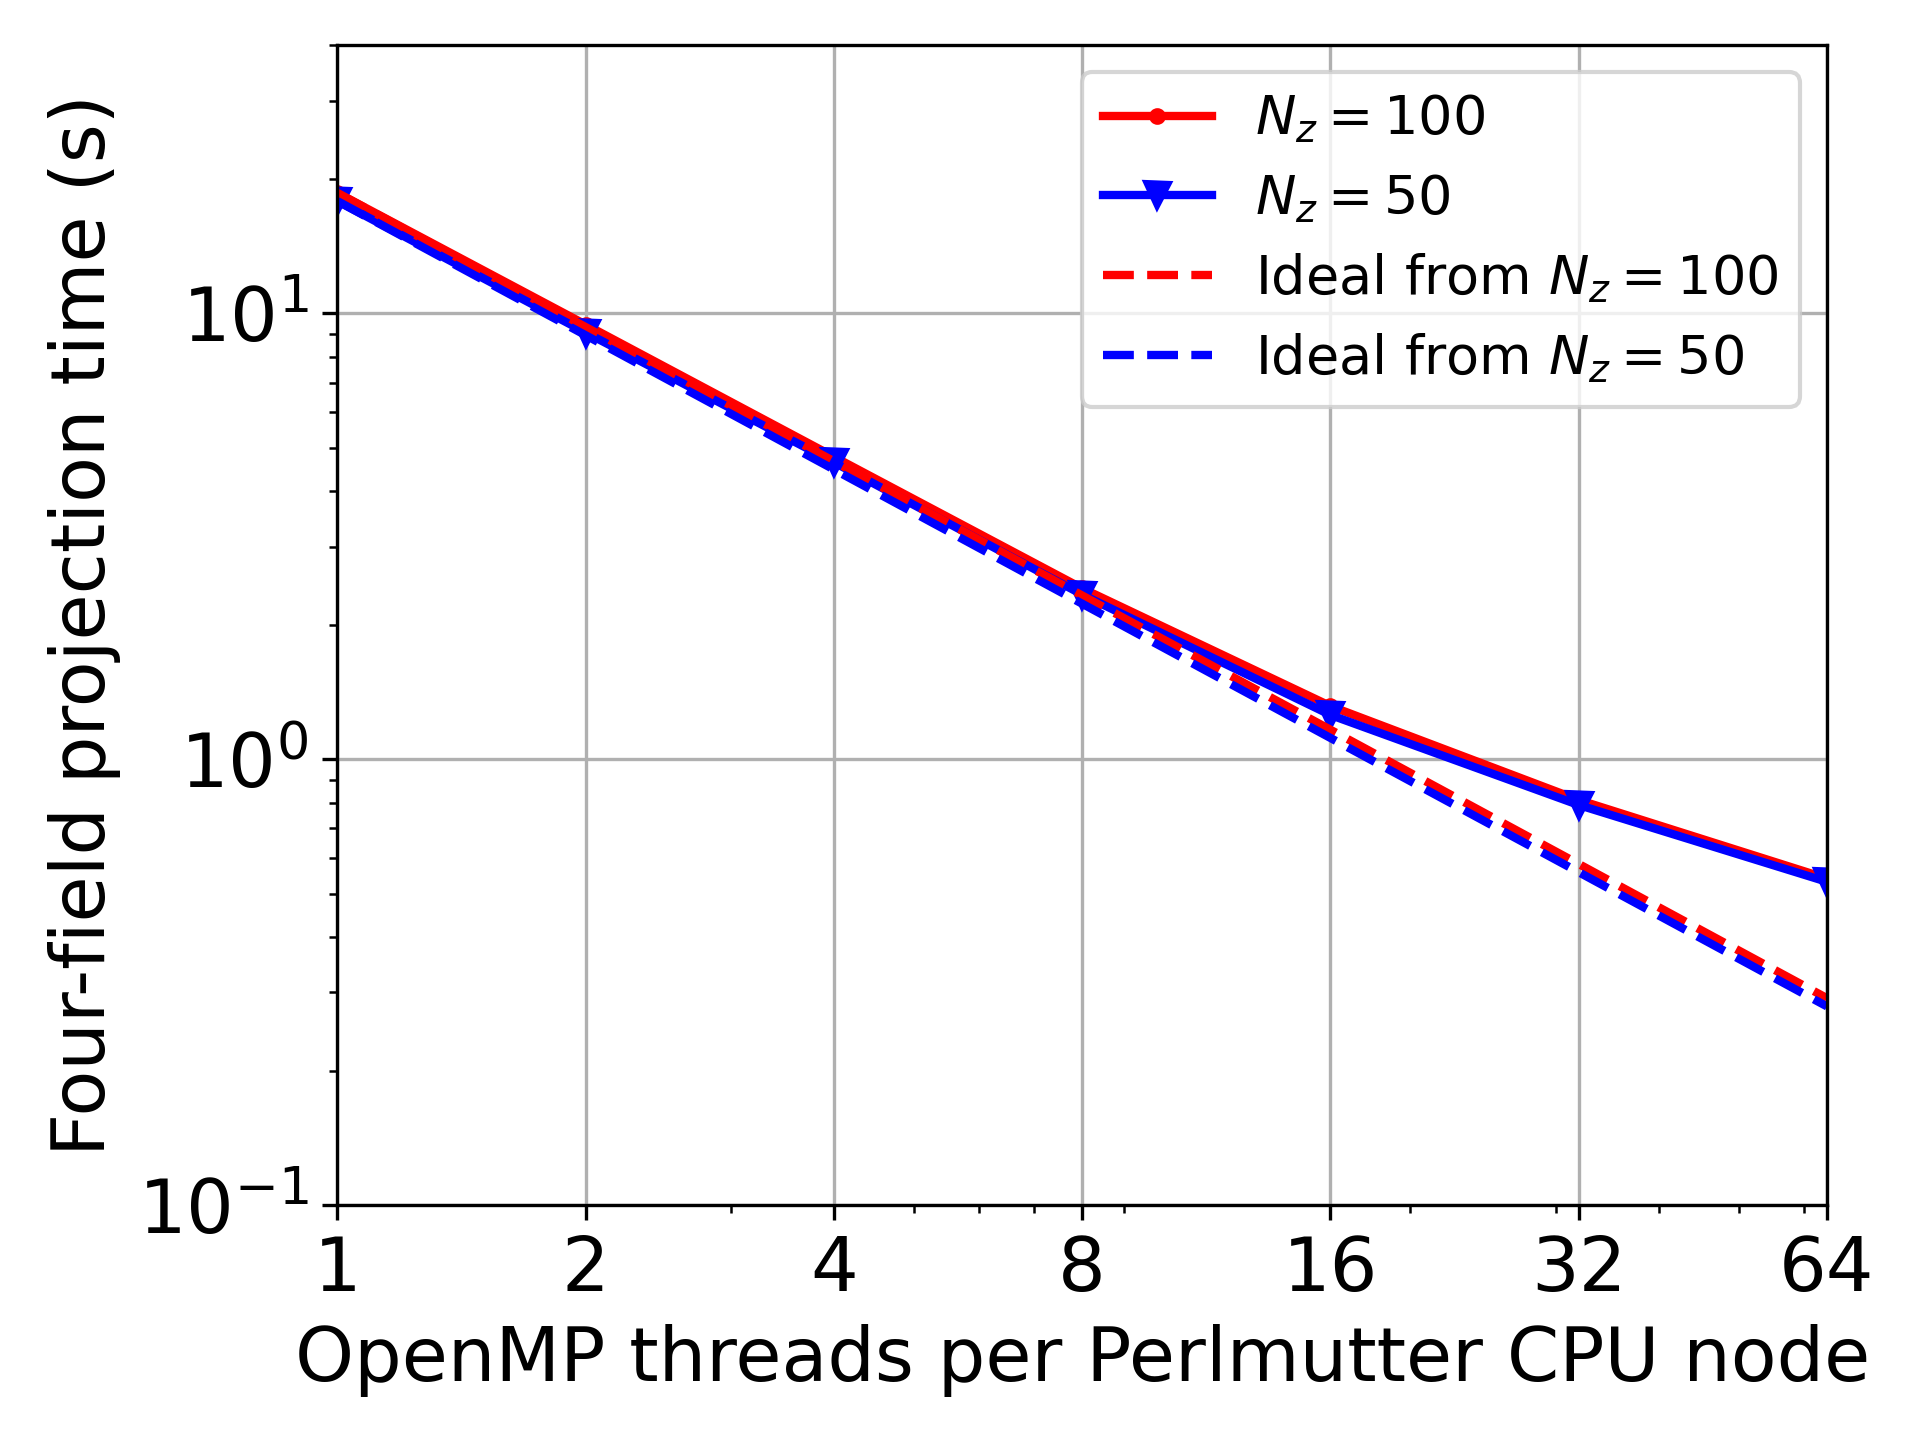
\includegraphics[width=0.7\textwidth]{Figures/conv_omp_scaling_perlmutter.png}
%\caption{Strong scaling of the four-field projection at $N_z=50$ and $N_z=100$.}
%\label{conv:fig:omp-scaling}
%\end{figure}
%\FloatBarrier
%
%Figure~\ref{conv:fig:omp-scaling} shows a measured speedup of $34.5\times$ at $N_z=100$ and $33.6\times$ at $N_z=50$, corresponding to an average of 53\% strong-scaling parallel efficiency at 64 threads, while the two vertical-resolution curves nearly overlap. The resuls for the run are averaged over 10 executions, and showcase the net volumetric remapping speedup rather than separately quantifying the cost of the horizontal and vertical phases of the remap.

\subsection{Bathymetry treatment and regional applications}\label{conv:sec:bathysmooth}
The projected bathymetry can generate sigma-coordinate pressure-gradient errors over steep slopes~\citep{haney1991pressure,mellor1994pressure}. We condition it with a one-ring log-depth averaging smoother. Writing $H_i$ for the depth of \ROMS cell $i$, $q_i=\log H_i$ for its logarithm, $\mathcal{A}(i)$ for the set of edge-neighbours of that cell, and $m$ for the iteration counter, each sweep replaces the log-depth of a cell by the mean over its one-ring neighbourhood,
\begin{equation}
 q_i^{(m+1)}=\frac{1}{|\mathcal{A}(i)|}\sum_{i'\in\mathcal{A}(i)}q_{i'}^{(m)},\qquad H_i^{(m+1)}=\exp q_i^{(m+1)},
 \label{conv:eq:onering}
\end{equation}
with clipping to the \MPAS range. Operating on $\log H$ rather than $H$ makes the smoother act on relative rather than absolute depth differences, so a given number of sweeps has comparable effect on the shelf and in the deep ocean. Land cells are excluded from the neighbourhood sums. Smoothing by Eq.~\eqref{conv:eq:onering} stops once the steepest remaining neighbour contrast satisfies
\begin{equation}
 r_{\max}^{(m)}=\max_i\max_{i'\in\mathcal{A}(i)}\frac{q_i^{(m)}-q_{i'}^{(m)}}{q_i^{(m)}+q_{i'}^{(m)}}<0.05,
 \label{conv:eq:slope-stop}
\end{equation}
which is the sole termination condition, with no cap on the iteration count. Evaluated on the same log-depths, this test plays the role of the $r$-factor conventionally used to condition terrain-following grids~\citep{sikiric2009smoothing}. The resulting bathymetry is shown in Fig.~\ref{conv:fig:smoothing}.

\begin{figure}[htbp]
\centering
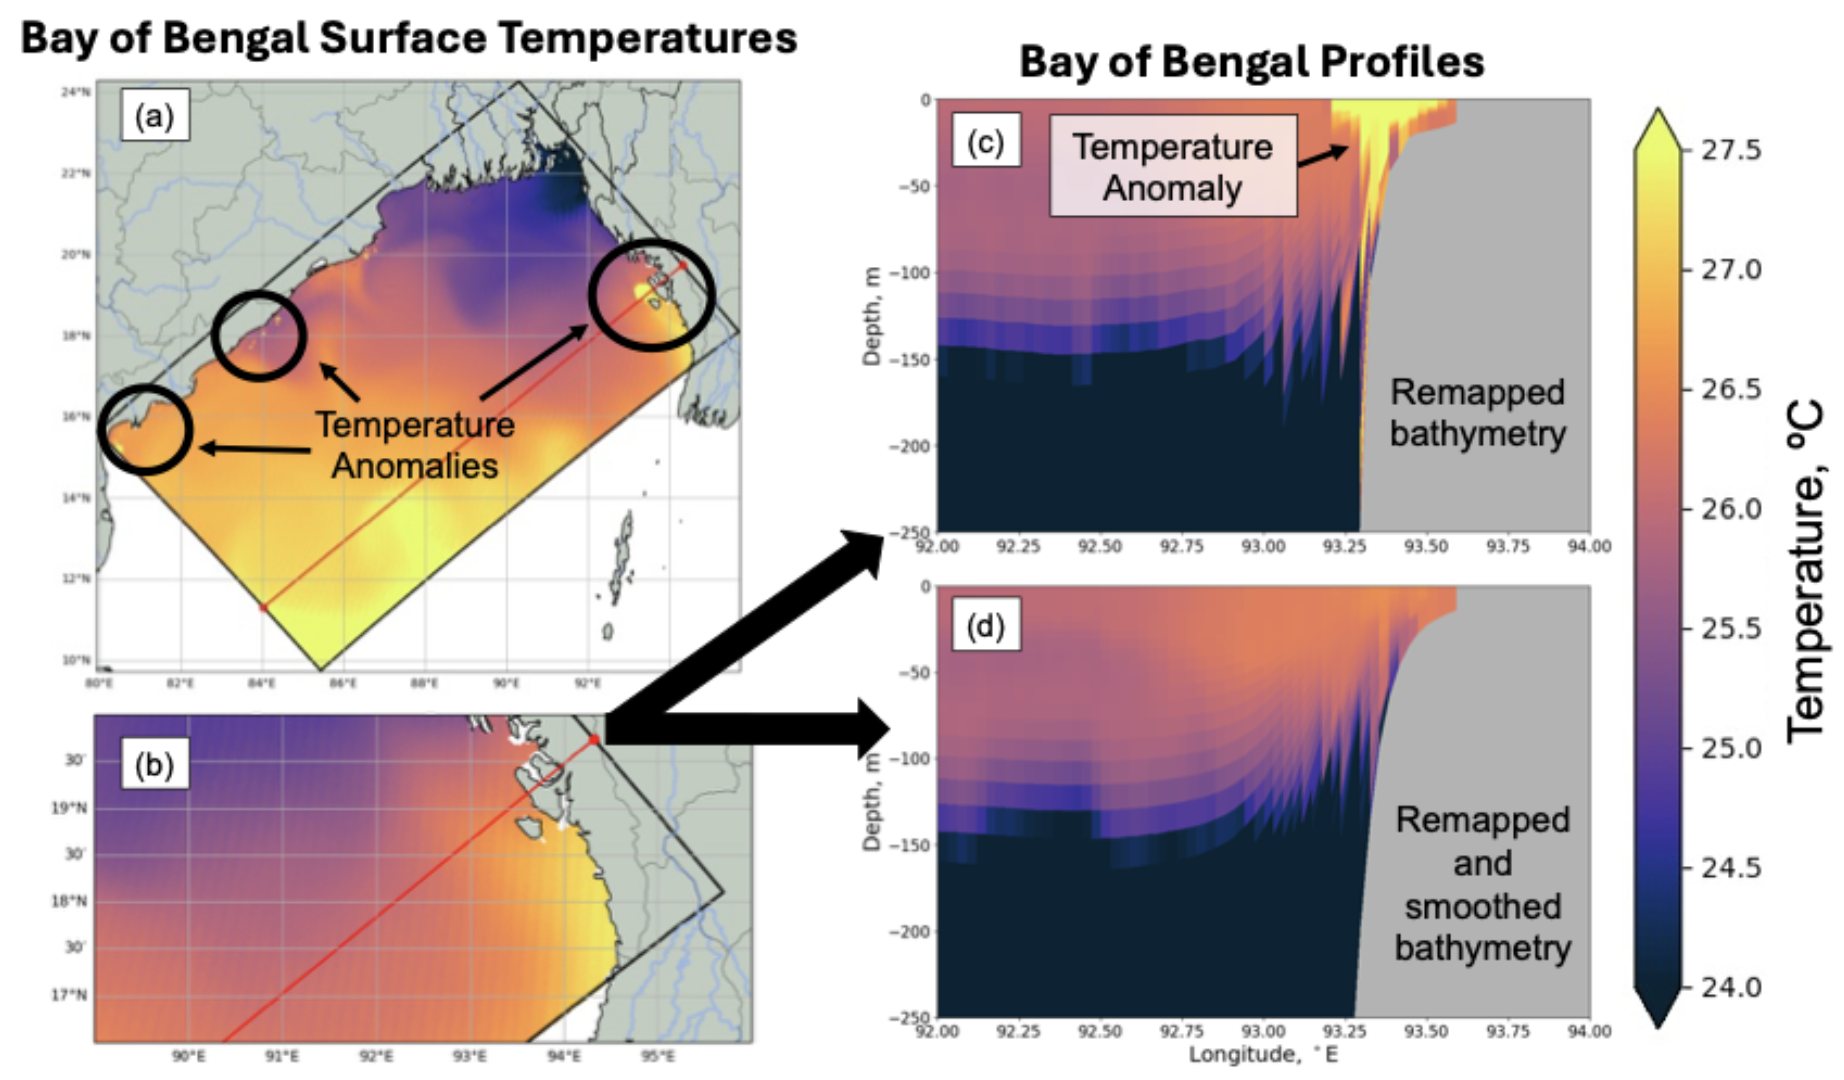
\includegraphics[width=\textwidth]{Figures/conv_bathy_smoothing.png}
\caption{Projected Bay of Bengal bathymetry before and after smoothing.}
\label{conv:fig:smoothing}
\end{figure}
\FloatBarrier

Smoothing the logarithm of the bathymetry changes the round-trip errors by less than 5\% and was sufficient to stabilize the Bay of Bengal integration. That domain also required vertical smoothing of the remapped scalar profiles, which removed a warm anomaly between 100 and 200 m near masked coastlines. The two treatments act on different quantities and we report their effects separately. Elsewhere the regional applications use the projected \MPAS geometry, except where coastal or estuarine topography forces us to blend it with the native \ROMS bathymetry and to retain the \ROMS land mask. Chesapeake Bay is the clearest example: the \MPAS mesh cannot represent the estuarine geometry at all, so the boundary and initial fields there must be prescribed or blended, and the blending weights we used are not specified precisely enough for the case to be reproduced.


Running \ROMS on finer regional meshes with \MPAS-derived boundary conditions produces finer-scale spatial variability across the regional domains (Fig.~\ref{fig:zeta_snapshots}). The kinetic-energy records change relative to the parent and directly remapped states in a domain-dependent way (Fig.~\ref{fig:region_KE}), reflecting both the transferred state and the variability generated by the regional dynamics. Chesapeake Bay is shown separately in Fig.~\ref{fig:chesResults} because its estuarine geometry requires blending. \REVIEWc{Kyle} The figures in this subsection illustrate what the downscaled simulations produce and they clearly show that submesoscale processes are born, evolve and propagate under regional refinements, which are averaged over by the global coarse scale models. \TODOc{add more}

\begin{figure}[htbp]
\centering
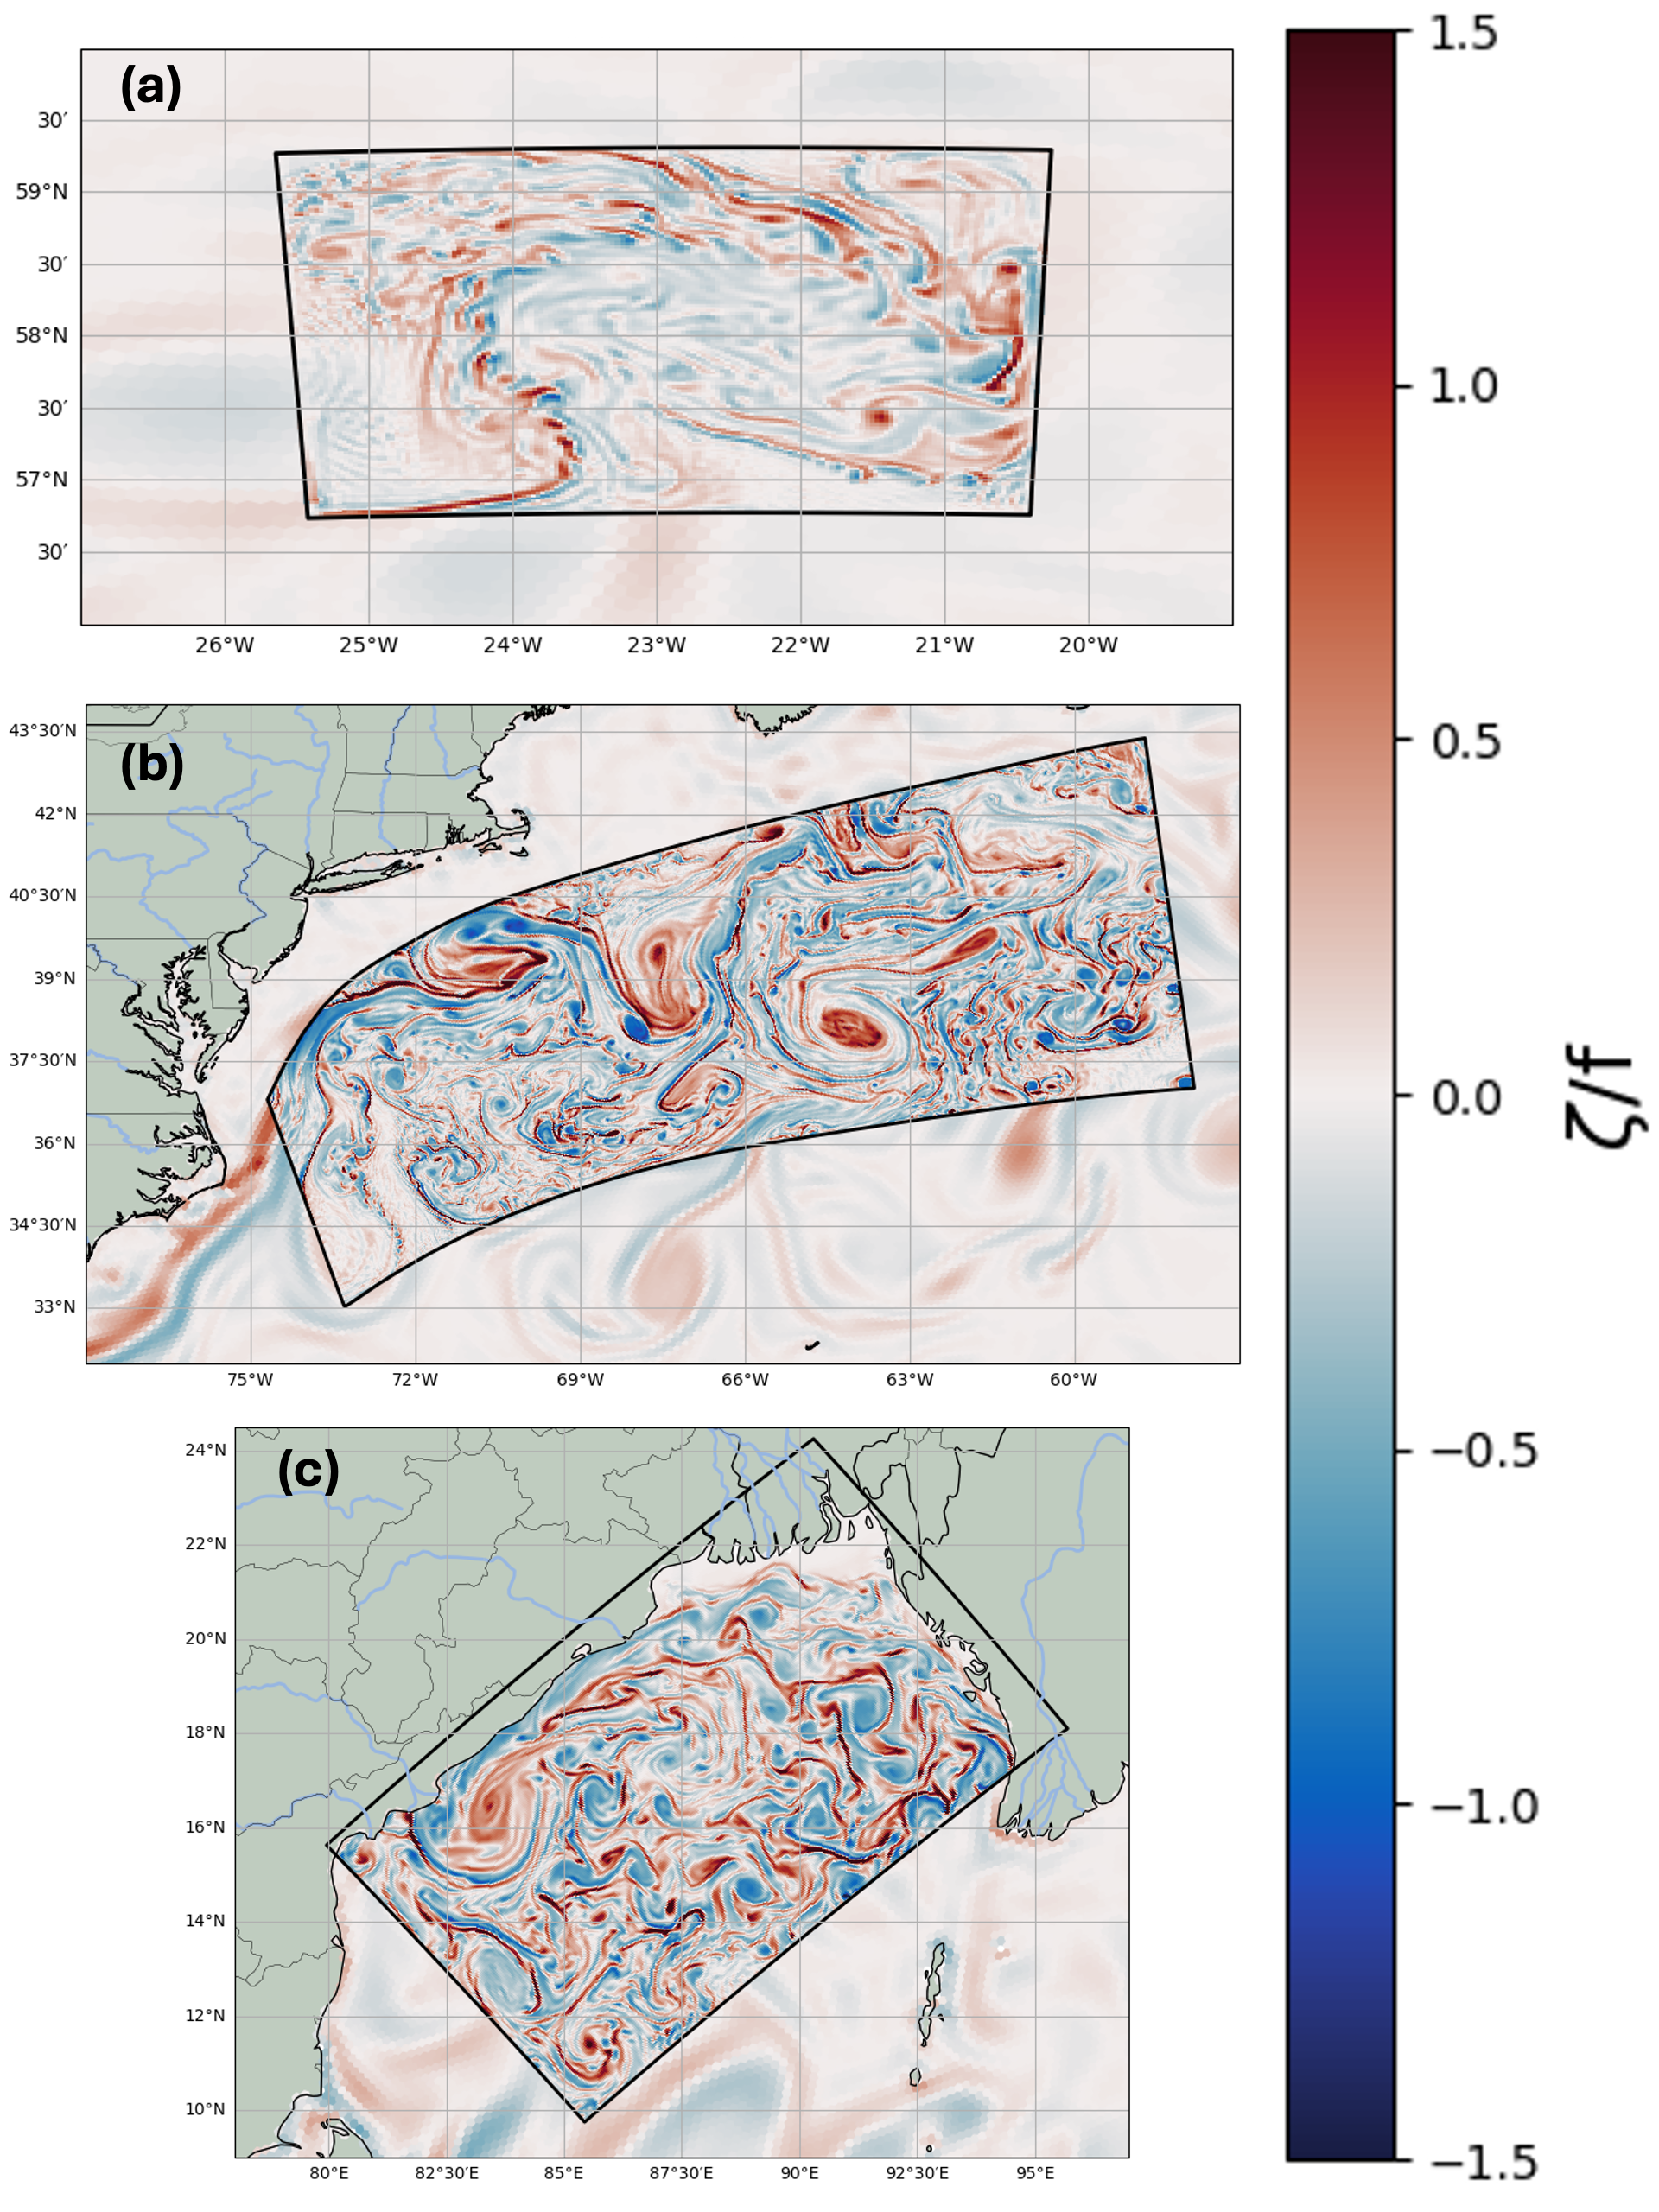
\includegraphics[width=0.90\textwidth]{Figures/zeta_3domains_v0.png}
\caption{Surface relative-vorticity fields for the North Atlantic, Gulf Stream, and Bay of Bengal regional domains.}
\label{fig:zeta_snapshots}
\end{figure}

\TODOc{Introduce and talk about benchmarks for regional domains and how these are validated}


\begin{figure}[htbp]
	\centering
	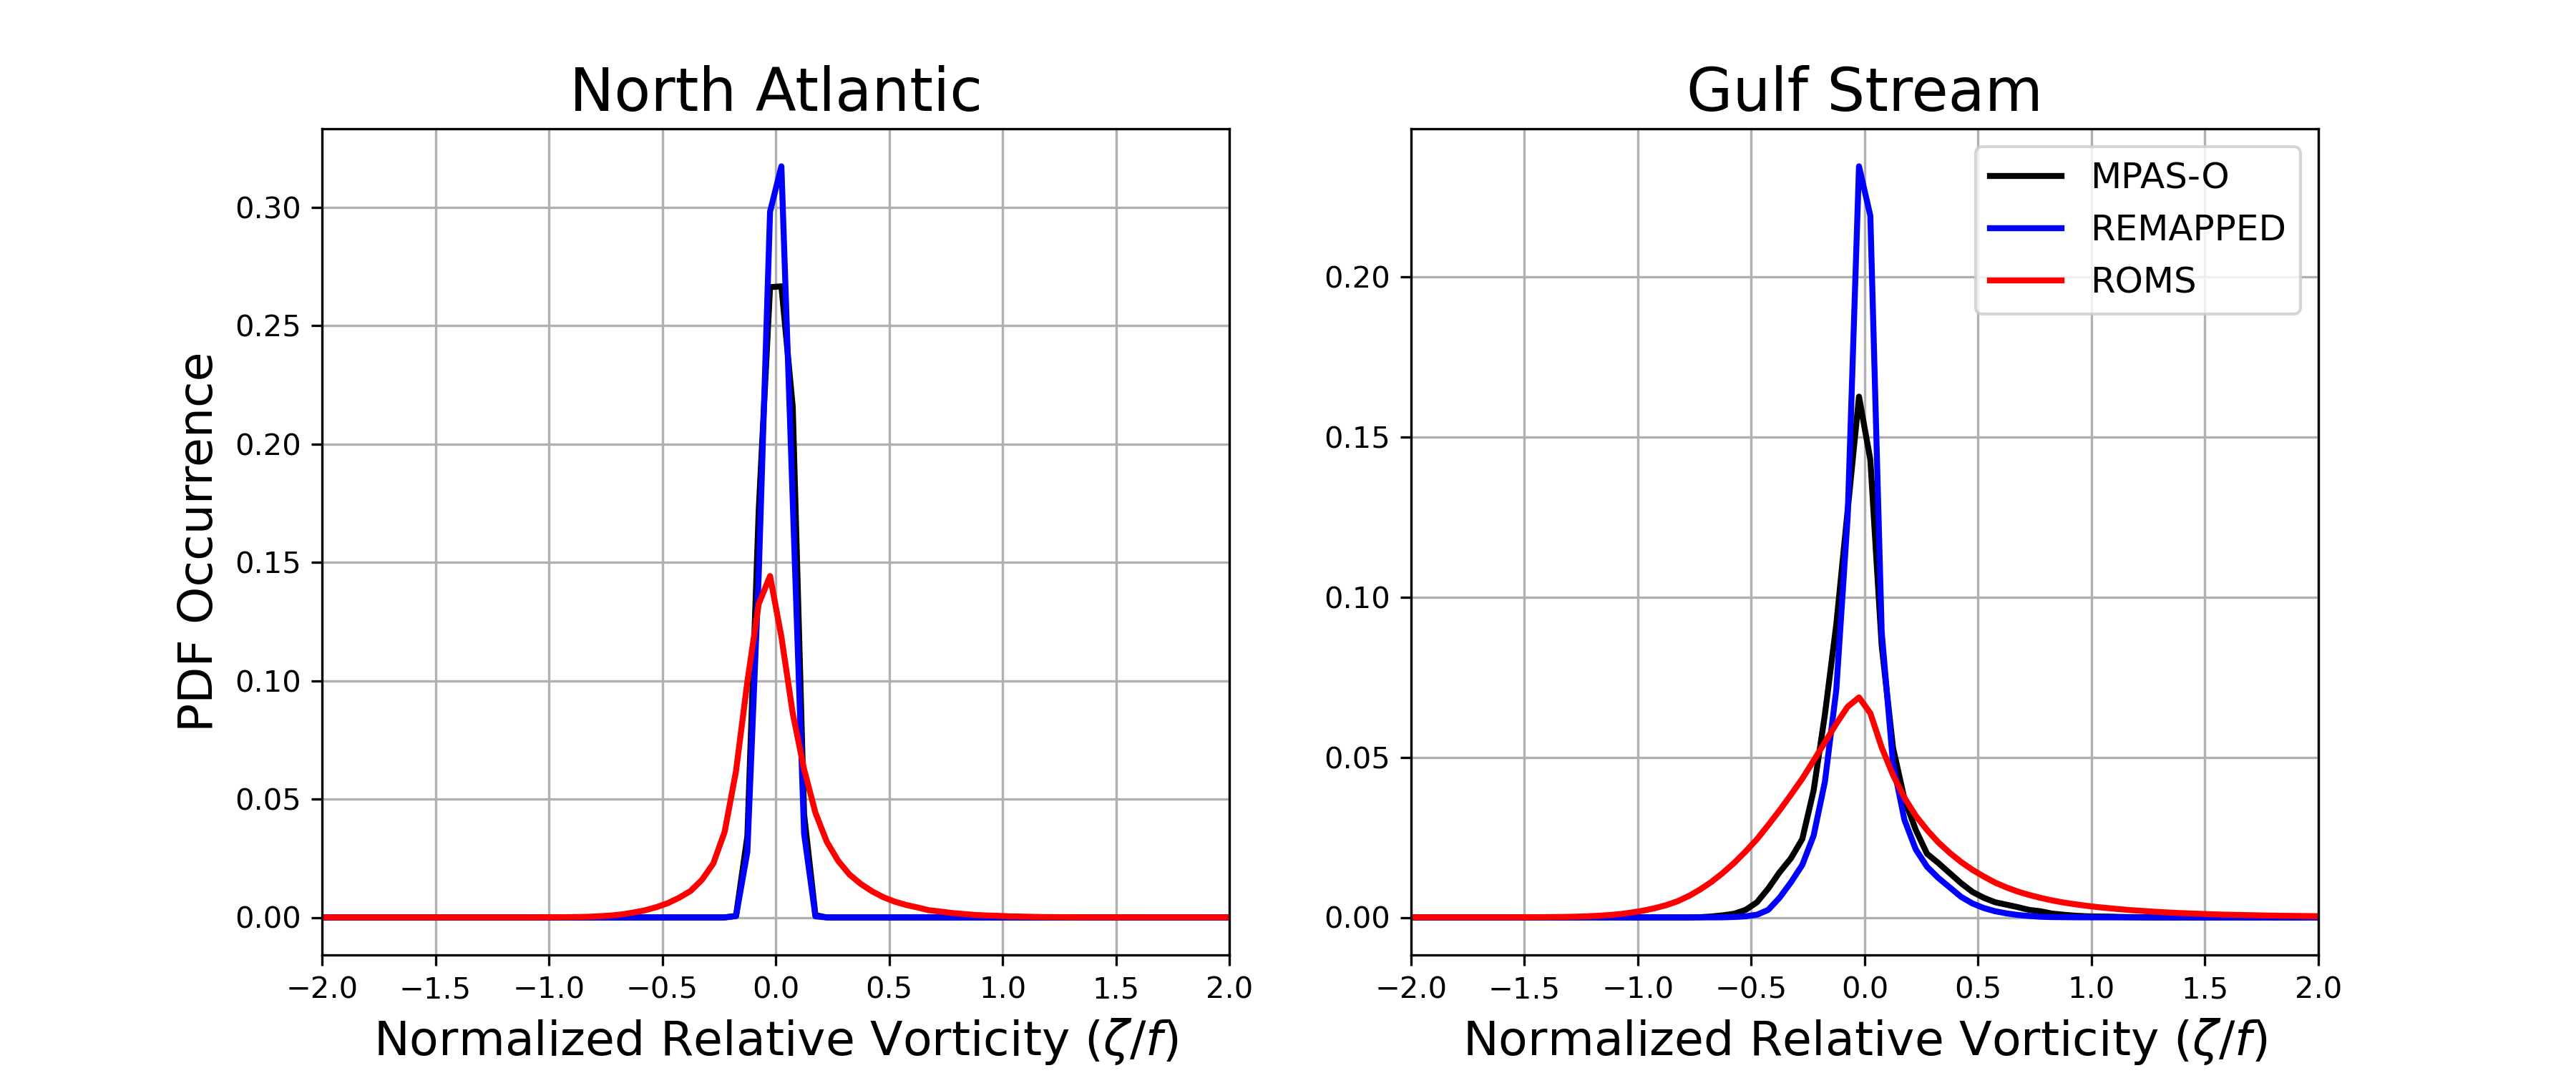
\includegraphics[width=0.88\textwidth]{Figures/regional_zeta.png}
	\caption{Normalized relative vorticity distribution for Niskine and Gulfstream cases.}
	\label{fig:relVortPDF}
\end{figure}
\FloatBarrier


The surface kinetic energy used in Fig.~\ref{fig:region_KE} is defined by
\begin{equation}
  \mathrm{KE}=\frac{1}{2}\left(u^2+v^2\right)\quad [\si{\metre\squared\per\second\squared}],
  \label{conv:eq:ke}
\end{equation}
with velocities represented at cell centers for the diagnostic.

\begin{figure}[htbp]
\centering
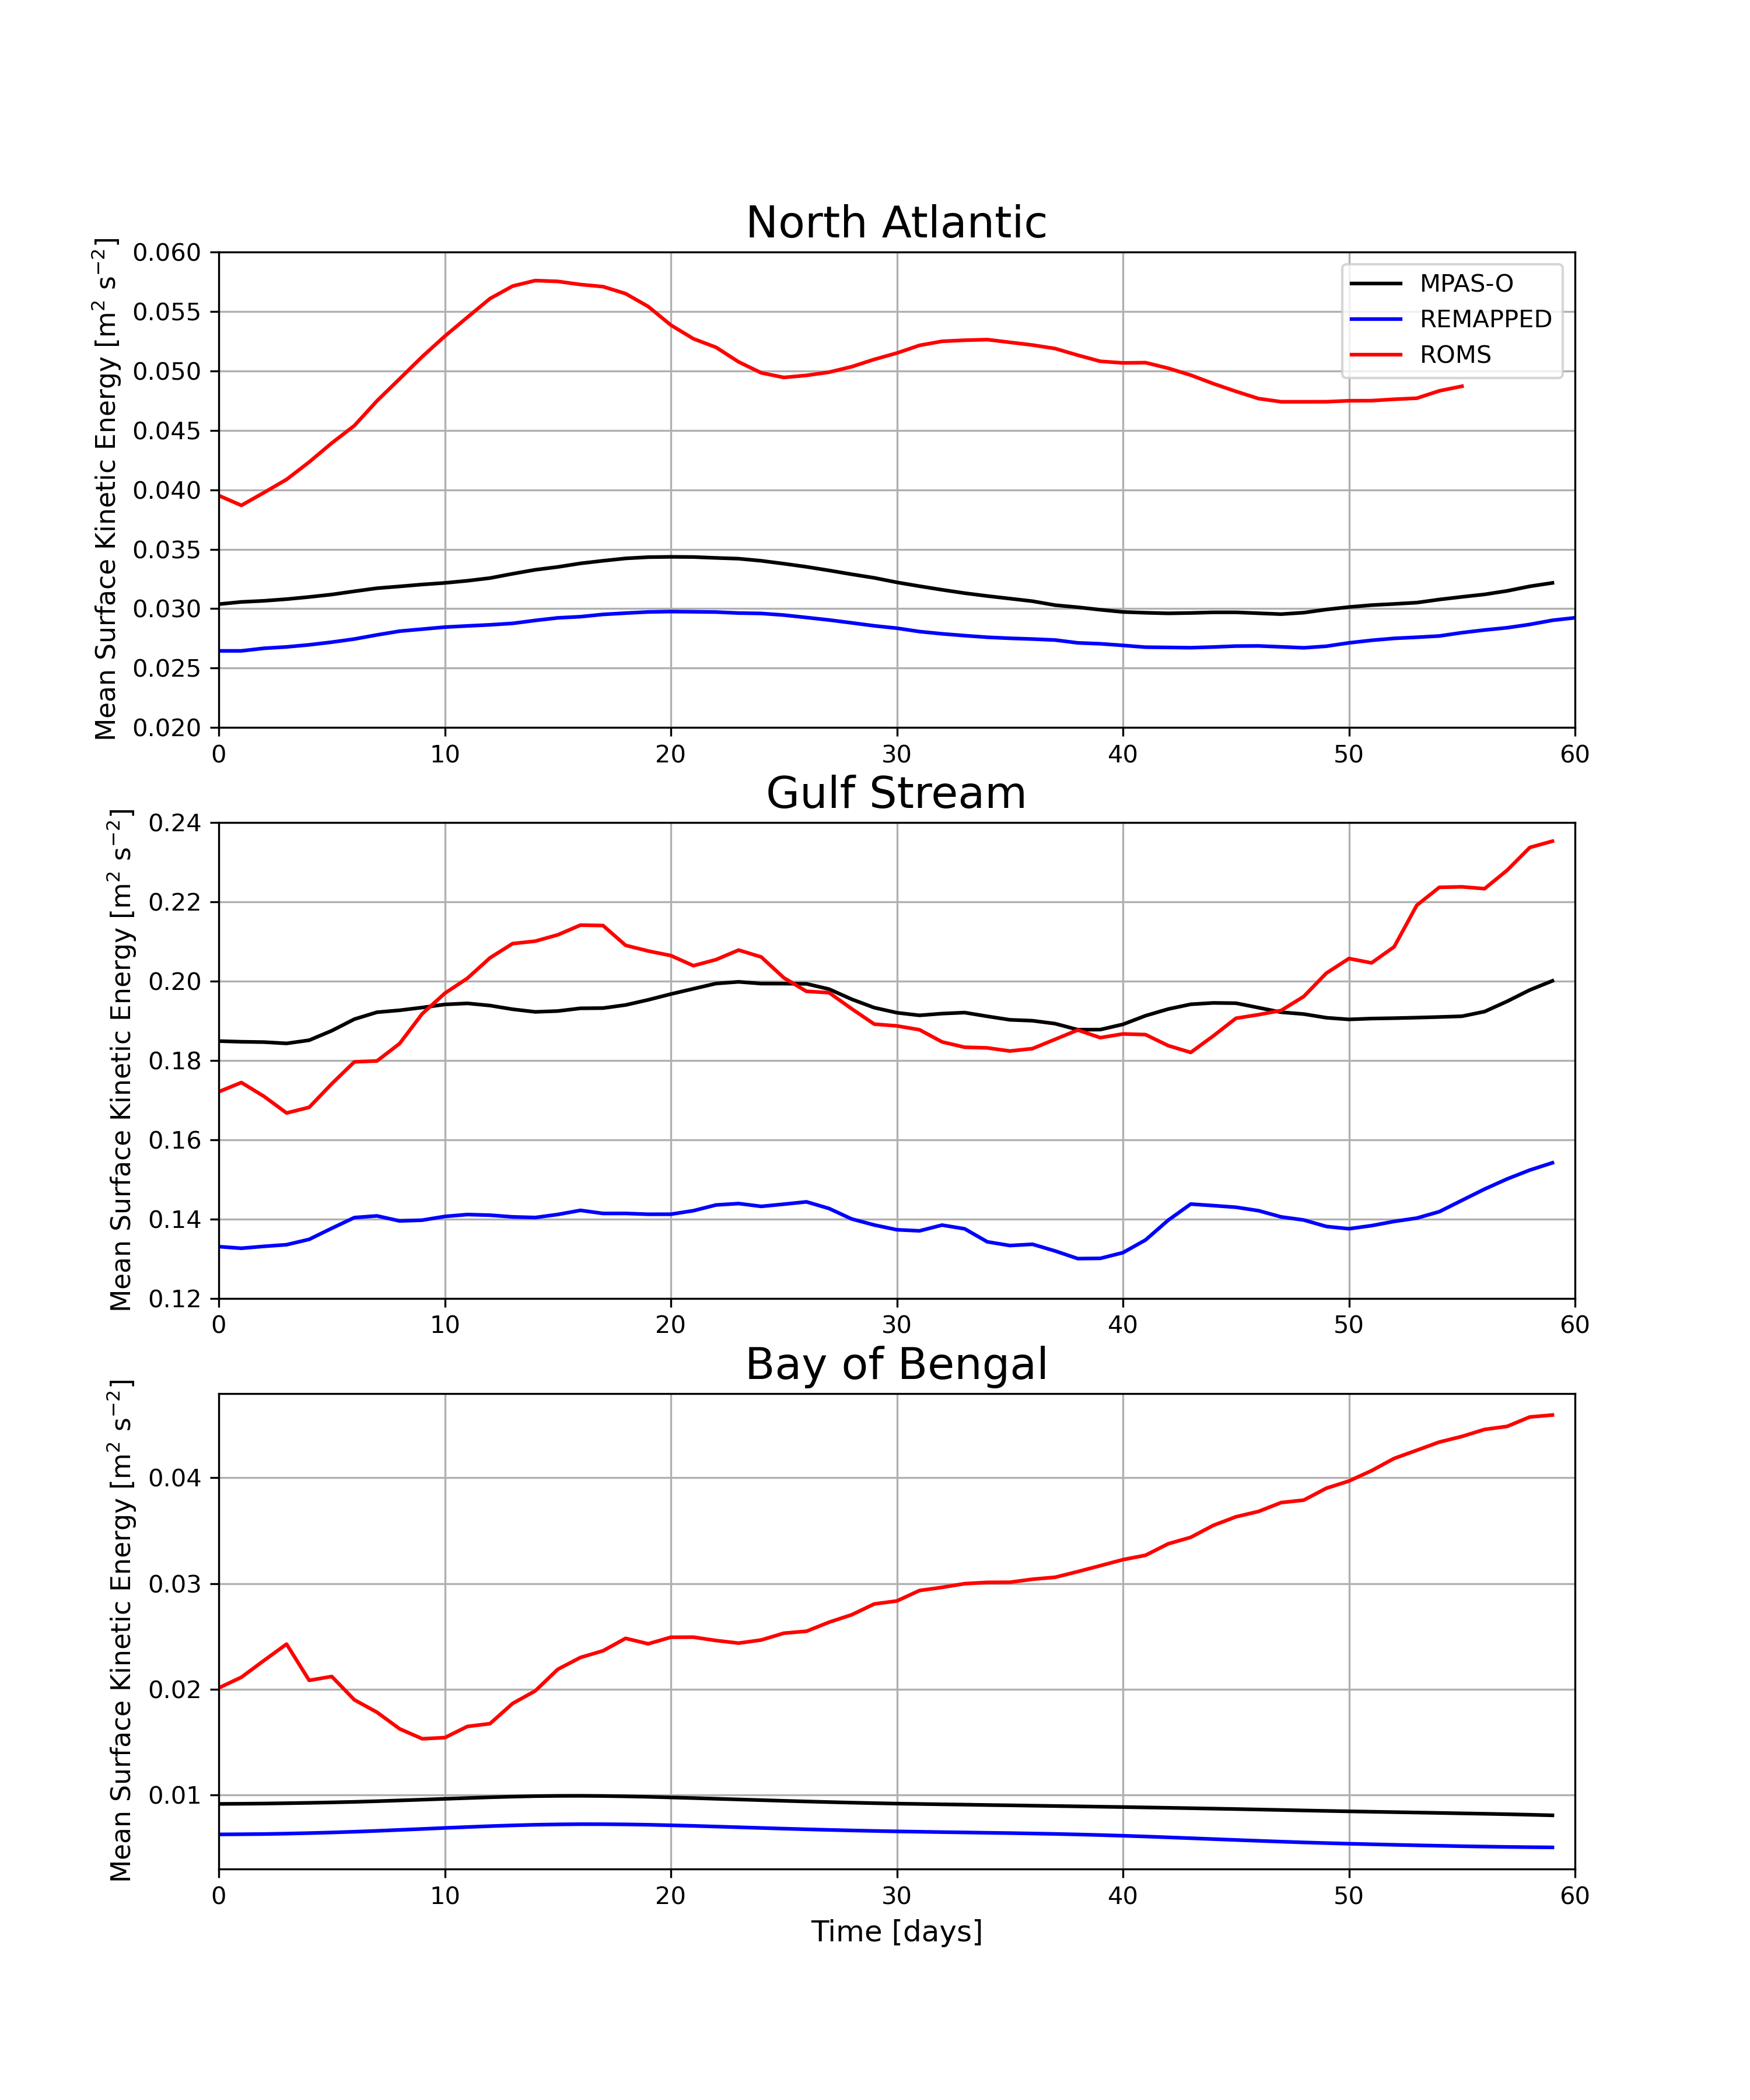
\includegraphics[width=\textwidth]{Figures/Region_KE_TimeSeries_3domains.png}
\caption{Surface specific kinetic-energy time series for the North Atlantic, Gulf Stream, and Bay of Bengal domains, evaluated with the diagnostic definition in Eq.~\eqref{conv:eq:ke}.}
\label{fig:region_KE}
\end{figure}

\begin{figure}[htbp]
\centering
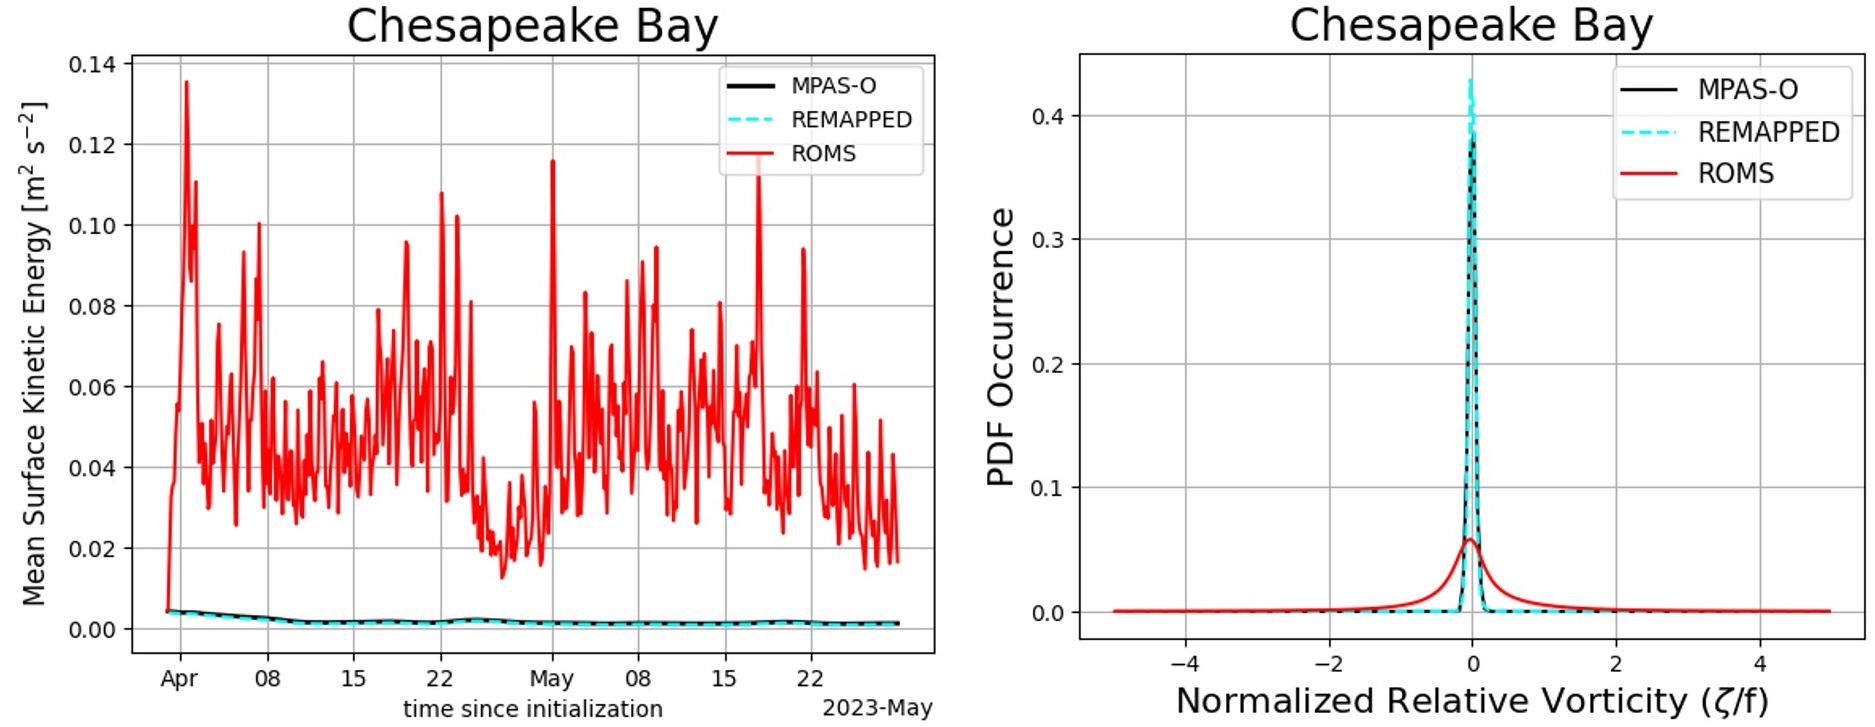
\includegraphics[width=0.88\textwidth]{Figures/chesbay_ke_zeta.jpg}
\caption{Surface specific kinetic energy and relative-vorticity distribution for Chesapeake Bay. These estuarine results are preliminary.}
\label{fig:chesResults}
\end{figure}
\FloatBarrier

The open-ocean and coastal applications occupy relative target scales near $\hRatio\approx0.2$--$0.35$, whereas Chesapeake Bay is substantially finer relative to its parent. In every domain the regional solution alters both the geometry of the flow and its energy content relative to the parent state. Because the regional model continues to evolve after initialization, these differences measure the combined effect of the transfer and the subsequent regional dynamics, and the convergence experiments of Sect.~\ref{conv:sec:conv} remain the quantitative statement about the transfer itself. The Chesapeake result depends particularly strongly on native bathymetry, land-mask treatment, and the blended estuarine fields. \TODOc{talk more about practical implementation of this case}


%

\FloatBarrier
\section{Discussion}\label{sec:discussion}

The transfer improves over the coarse portion of the tested sequences, but its composite round-trip error saturates for real fields on the finest pair. For the controlled analytic field, refining the \ROMS mesh while holding \MPAS fixed shows that the \ROMS characteristic length is not what limits the result, while cancellation between the forward and reverse legs makes the round trip a different quantity from the one-way forcing error. Which stage sets the floor remains unattributed, since we did not exercise the horizontal and vertical operators separately. Requiring the vertical interpolant to conserve layer integrals makes the composed tensor-product transfer first order overall, which is consistent with the measured decrease, though confirming the rate by fitting would require a longer sequence than the four grids used here.

The regional applications show finer-scale relative-vorticity structure and domain-dependent kinetic energy changes across open-ocean, boundary current, coastal, and estuarine settings. The four configurations sit at $\hRatio\approx0.21$ (North Atlantic), $0.24$ (Gulf Stream), $0.35$ (Bay of Bengal), and $0.06$ (Chesapeake Bay), so three of them lie near the flattening point identified in \S\ref{conv:sec:conv} while Chesapeake Bay is far below it, refined for reasons of estuarine geometry rather than transfer accuracy. As a result, the Chesapeake Bay case utilizes blended bathymetry information to produce better fidelity in regions where \MPAS can only provide sparse data.

Several limitations qualify some of these presented results. The \MPAS characteristic length is fixed and varies in space, while the \ROMS evaluation support changes as that mesh is refined (depending on the interior set, $\mathcal{I}$). Additionally, velocities are transferred between \MPAS and \ROMS models as componentwise scalars, and remain cell centered, without rotation to the \ROMS curvilinear basis, interpolation to staggered points, or any constraint on the discrete divergence. Future studies should explore use of Mimetic schemes to achieve edge-based, high-order consistent projections that do not require 3 levels of remapping to transfer velocity fields from unstructured \MPAS to \ROMS. 

It is important to bear in mind that neither finer \ROMS meshes nor higher-order interpolation schemes can remove the errors imposed by a coarse \MPAS representation in regions that require higher fidelity for better boundary forcing, definition of land masks, or estuarine structures. We have performed the resolution verification study to identify optimal characteristic length resolution, which can guide future efforts to improve resolution in regions of interest when designing CVT refinements for the \MPAS global ocean model.

\TODOc{add more relevant discussions from real world one-way runs; can reference videos of tracer evolution and discuss the chesapeake case and how that was achieved. Complications in getting that to work and why this augments global models.}

\TODOc{Placeholder for graph neural network exploration for volumetric remapping with conservation and monotonicity constratints}
%

%

\FloatBarrier
\section{Summary and future directions}\label{sec:conclusions}
%
%
\TODOc{Revise conclusion sections fully - later}
We present a separable volumetric transfer for models with different horizontal meshes and vertical coordinates. The method combines a consistent horizontal remap with a column-wise conservative vertical projection that reproduces \ROMS layer integrals. Because the vertical operator is constrained to preserve these integrals, the composite method is first-order accurate. In the one-dimensional tests, a non-conservative point-value interpolant reproduced smooth profiles with convergence between second and third order, but renders the method non-conservative. 

For practical applications, a \ROMS{}-$\rightarrow$-\MPAS{} resolution ratio of approximately \(\hRatio \approx 0.2\) provides a useful initial target. This value should be tested through a short refinement sequence for each domain rather than adopted as a universal threshold. The case studies also show that remapping alone is insufficient to produce a viable regional configuration. The Bay of Bengal simulation required bathymetric smoothing, while Chesapeake Bay required native estuarine geometry and blended fields in addition to the \MPAS forcing conditions.

Two additional tests would most directly strengthen the verification. First, comparing real fields over their common support on the finest available grid pair would determine whether the apparent error saturation reflects the transfer itself or changing coverage between resolutions. Second, isolated tests of the vertical remapper on synthetic columns would establish its convergence behavior independently of horizontal interpolation and changing wet-domain support. These tests should include cases in which the ROMS water column is contained within, matches, or exceeds the \MPAS depth range. Further evaluation could include forward-transfer tests for physical tracers against surrogate reference solutions, sensitivity experiments using multiple \MPAS meshes, and repeated timing measurements. Together, these tests would provide a stronger basis for evaluating online one-way coupling.

The same framework can support two-way coupling. The roundtrip analysis already requires reverse horizontal and vertical operators, \(W_{R\to M}\) and \(\mathcal{V}_{R\to M}\), in addition to the forward maps. The tensor-product formulation can therefore be applied with ROMS as the source and \MPAS as the target, transferring regional information back to the global mesh.
%What the round trip does not do is validate that reverse leg on its own, because errors incurred on the forward leg can be undone on the return, and the composition is therefore a weaker test than either direction taken separately. 
The numerical considerations differ in the upscaling direction. Fine-to-coarse transfer aggregates many \ROMS cells into a single \MPAS cell, rather than distributing one coarse \MPAS value across many fine \ROMS cells. Consequently, mesh imprinting is not the principal concern, and high-order conservative \(L_2\)-minimization  horizontal transfer can be used without producing the staircase artifacts that motivated use of quasi-interpolatory maps like the normalized bilinear interpolation for downscaling. 



\FloatBarrier
\section*{Data and Code Availability}
\TODOc{Availability: Replace with complete data and method access information.}
%

\FloatBarrier
\section*{Acknowledgments}
\TODOc{Acknowledgments: Replace with funding and computing acknowledgments.}
%

\clearpage
\bibliographystyle{ametsocV6}
\bibliography{references}
%%

\end{document}
